\chapter{Ergebnisse der Berechnung}
\label{chap:berechnung}
% Inhalt (Gliederung Kapitel 5, etwa 12 S.).

\section{Faserorientierung aus der Spritzgießsimulation}
\label{sec:faserorientierung}

Die Faserorientierung der Spritzgießsimulation wurde über das CONVERSE-Mapping nach \secref{sec:fe_modell} auf das FE-Netz übernommen und am Zahn T3 des Sektors so ausgewertet, wie der Forschungsbericht FVA 856 I seine Computertomographie auswertet \cite[Kapitel~6.2 und 6.3]{FVA856-I}. Je Element wird der Orientierungstensor aus dem Faserrahmen und den beiden größten Eigenwerten gebildet, je Zone das volumengewichtete Mittel. Daraus folgen die Eigenwerte $\lambda_{1} \le \lambda_{2} \le \lambda_{3}$, der Anisotropie-Index $AI = 1 - \lambda_{1}/\lambda_{3}$ und die Vorzugsrichtung in der Stirnebene. Die Zonen folgen Bild 17 des Berichts mit dem Randstreifen bis $0{,}2$\,mm unter der Kontur, dem Übergangsstreifen bis $0{,}4$\,mm und darunter dem Kern M über dem Fußkreis und U darunter. \figref{fig:faserorientierung_schnitt} zeigt die Faserrichtung je Element in zwei Stirnschnitten, \figref{fig:faserorientierung_zonen} die Zonen mit der simulierten Vorzugsrichtung.

\begin{figure}[htbp]
    \centering
    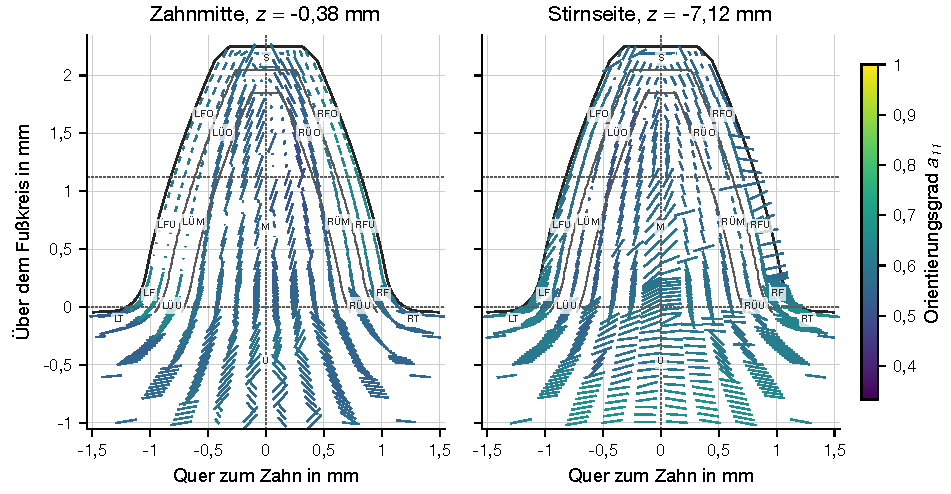
\includegraphics[width=\textwidth]{kap5/faserorientierung_schnitt}
    \caption{Faserrichtung je Element in zwei Stirnschnitten des Zahns T3 (Zahnmitte und Stirnseite): Linienrichtung ist die Hauptachse der Orientierung, die Farbe der Orientierungsgrad $a_{11}$. Zonen und Streifen von $0{,}2$\,mm in Anlehnung an \cite[Bild~15 und 17, S.~17 und 19]{FVA856-I}.}
    \label{fig:faserorientierung_schnitt}
\end{figure}

\figref{fig:faserorientierung_schnitt} zeigt, dass die Orientierung über der Zahnbreite nicht gleich ist. In der Zahnmitte liegen die Fasern der Flanken- und Kopfzonen axial, ihre Hauptachse steht fast senkrecht auf der Stirnebene, so dass die Linien dort kurz erscheinen. Im Kern M und unter dem Fußkreis laufen sie radial entlang der Zahnachse. An der Stirnseite folgen die Fasern dagegen in allen Randzonen der Kontur in der Stirnebene, mit langen Linien entlang der Flanke und um den Fuß. Im Kern verwirbeln sie ohne Vorzugsrichtung, unter dem Fußkreis liegen sie tangential. Der Orientierungsgrad $a_{11}$ liegt in beiden Schnitten zwischen $0{,}5$ und $0{,}7$, am höchsten in den Fußzonen und unter dem Fußkreis. Die Zonenwerte der folgenden Absätze sind Mittel über die ganze Breite und mischen beide Bilder.

% TK erledigt (Absatz zu Bild 5.1 ergänzt): Zu wenig oder gar nichts zu Bild 5.1 gesagt, obwohl da schön zu erkennen ist, dass sich die Orientierung über der Zahnbreite unterschiedet.

\begin{figure}[htbp]
    \centering
    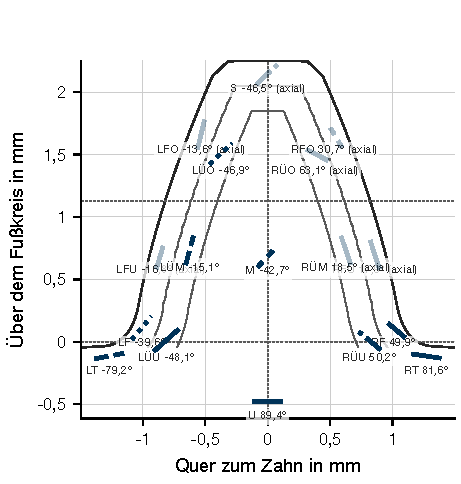
\includegraphics[width=0.9\textwidth]{kap5/faserorientierung_zonen}
    \caption{Zonen des Zahns T3 mit der Vorzugsrichtung der Simulation in der Stirnebene, in Anlehnung an \cite[Bild~18, S.~19]{FVA856-I}.}
    \label{fig:faserorientierung_zonen}
\end{figure}

% TK erledigt (Bild kleiner, Beschriftungen entzerrt, Legende ergänzt): Die Grafik gefällt mir nicht. Zu groß auf dem Blatt dargestellt und innerhalb der Grafik überlappen sich einige Beschriftungen. Sieht nicht so qualitätiv hochwertig aus, wie Bild 5.1 und eine Legende fehlt auch.

\tabref{tab:faserorientierung_zonen} stellt den Anisotropie-Index der linken Zonen dem CT-Befund gegenüber. Die rechten Zonen liegen innerhalb von $0{,}08$ bei den linken. Über die ganze Zahnbreite gemittelt sind die simulierten Fußrundungen und unteren Flanken mit $AI$ von $0{,}33$ bis $0{,}35$ weit weniger anisotrop als die CT-Zonen mit $0{,}83$ bis $0{,}86$. Die Übergangszonen liegen mit $0{,}20$ bis $0{,}35$ gegen $0{,}60$ bis $0{,}76$. Nahe beieinander liegen der Fußgrund mit $0{,}63$ gegen $0{,}71$, die obere Flanke mit $0{,}62$ gegen $0{,}76$, der Kern M mit $0{,}30$ gegen $0{,}35$ und U mit $0{,}67$ gegen $0{,}70$. Die Elemente selbst sind mit einem mittleren größten Eigenwert von $0{,}55$ bis $0{,}66$ deutlich orientiert. Das Zonenmittel verliert seine Anisotropie durch die Neigung der Faserachse. In beiden Hälften der Zahnbreite kippt sie mit entgegengesetztem Vorzeichen aus der Stirnebene, um $25$ bis $75$° im Drittel an der einen und um $45$ bis $69$° an der anderen Stirnseite. Dadurch heben sich die Nebendiagonalglieder auf. \figref{fig:faserorientierung_drittel} zeigt deshalb den Index je Drittel der Zahnbreite wie Bild 23 des Berichts. In den Dritteln erreichen Fußrundungen und Flanken $0{,}65$ bis $0{,}80$ gegen $0{,}76$ bis $0{,}86$ im CT, der Fußgrund $0{,}64$ bis $0{,}80$ gegen $0{,}71$ und die Übergangszonen $0{,}47$ bis $0{,}68$ gegen $0{,}60$ bis $0{,}76$. Das mittlere Drittel ist in Fußgrund, Fußrundungen, unteren Flanken und den meisten Übergangszonen weniger anisotrop als die äußeren Drittel. Sein $\lambda_{3}$ liegt um $8$ bis $27$\,\% tiefer. Der Bericht findet an seinem Rad $5$ bis $15$\,\% in den Außenzonen und bis $20$\,\% in den Übergangszonen \cite[Bild~23, S.~24]{FVA856-I}.

\begin{table}[htbp]
    \caption{Anisotropie-Index $AI$ und größter Eigenwert $\lambda_{3}$ der linken Zonen des Zahns T3: Spritzgießsimulation über die ganze Zahnbreite und im mittleren Drittel gegen die CT-Zonen des Forschungsberichts \cite[Bild~17 und 23, S.~19 und 24]{FVA856-I}. Vorzugsrichtung in der Stirnebene ($0$° Zahnachse, positiv nach links), \glqq axial\grqq{} wo die Hauptachse entlang der Zahnbreite liegt.}
    \label{tab:faserorientierung_zonen}
    \centering
    \footnotesize
    \begin{tabular}{L{3.4cm}L{1.3cm}L{1.3cm}L{1.6cm}L{1.3cm}L{2.0cm}L{2.0cm}}
        Zone               & $AI$ Sim. & $AI$ Mitte & $\lambda_{3}$ Sim. & $AI$ CT  & Richtung Sim. & Richtung CT \\
        \hline
        \arrayrulecolor{black!30}
        Fußgrund LT        & $0{,}63$  & $0{,}64$   & $0{,}53$           & $0{,}71$ & $-79$°        & $-82$°      \\
        \hline
        Fußrundung LF      & $0{,}34$  & $0{,}68$   & $0{,}40$           & $0{,}86$ & $-40$°        & $-28$°      \\
        \hline
        Flanke unten LFU   & $0{,}35$  & $0{,}71$   & $0{,}43$           & $0{,}83$ & axial         & $-13$°      \\
        \hline
        Flanke oben LFO    & $0{,}62$  & $0{,}75$   & $0{,}50$           & $0{,}76$ & axial         & $-19$°      \\
        \hline
        Kopf S             & $0{,}41$  & $0{,}35$   & $0{,}45$           & $0{,}55$ & axial         & $-89$°      \\
        \hline
        Übergang unten LÜU & $0{,}28$  & $0{,}59$   & $0{,}39$           & $0{,}76$ & $-48$°        & $-33$°      \\
        \hline
        Übergang Mitte LÜM & $0{,}20$  & $0{,}54$   & $0{,}37$           & $0{,}70$ & $-15$°        & $-33$°      \\
        \hline
        Übergang oben LÜO  & $0{,}25$  & $0{,}52$   & $0{,}37$           & $0{,}60$ & $-47$°        & $-33$°      \\
        \hline
        Kern M             & $0{,}30$  & $0{,}39$   & $0{,}39$           & $0{,}35$ & $-43$°        & $-85$°      \\
        \hline
        Kern U             & $0{,}67$  & $0{,}69$   & $0{,}49$           & $0{,}70$ & $89$°         & --          \\
        \hline
        \arrayrulecolor{black}
    \end{tabular}
\end{table}

\begin{figure}[htbp]
    \centering
    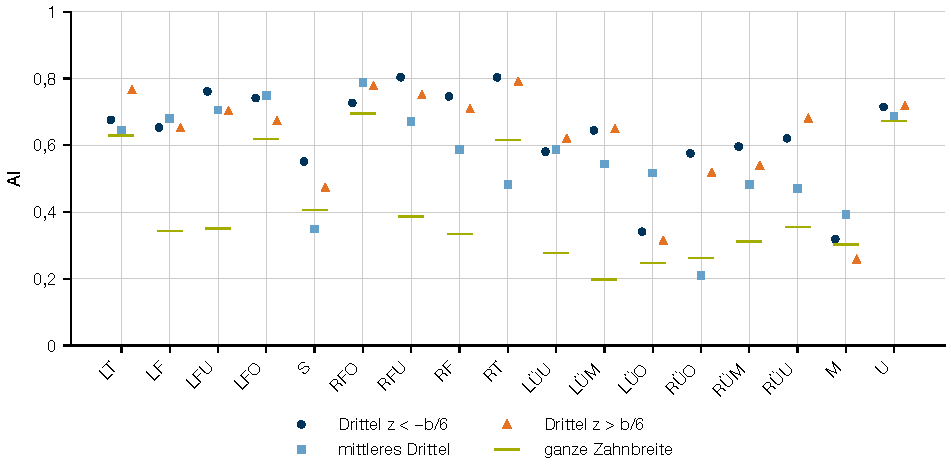
\includegraphics[width=\textwidth]{kap5/faserorientierung_drittel}
    \caption{Anisotropie-Index je Zone über die ganze Zahnbreite und in den Dritteln der Zahnbreite, in Anlehnung an \cite[Bild~23, S.~24]{FVA856-I}.}
    \label{fig:faserorientierung_drittel}
\end{figure}

In der Richtung stimmen Fußgrund und Kern U mit dem Bericht überein. Die Fasern laufen quer zum Zahn, mit $-79$ und $+82$° gegen $-81{,}6$ und $+84{,}4$°. Die Fußrundungen und unteren Übergangszonen liegen in der Stirnebene bei $-40$ bis $-48$° links und $+50$° rechts. Der Bericht nennt $-27{,}5$ und $+28{,}5$° für die Fußrundungen und $\mp 32{,}5$° für die Übergangszonen. Die Simulation liegt damit im selben Sinn, aber $12$ bis $21$° steiler. In den oberen Flanken, am Kopf und in der oberen rechten Übergangszone liegt die Hauptachse dagegen entlang der Zahnbreite. Ihr Anteil in der Stirnebene beträgt nur $0{,}01$ bis $0{,}06$, während das CT dort Fasern in der Ebene entlang der Oberfläche sieht. Der Kern M läuft in der Simulation bei $-43$° statt $-85$°. Die wahrscheinliche Ursache liegt in der Füllung. Der virtuelle Verteiler speist die Stegebene, Kranz und Zähne füllen von der Zahnmitte zu beiden Stirnseiten, so dass die Strömung im dünnen Zahn entlang der Breite läuft. Wie das Rad des Berichts angespritzt wurde, nennt dessen Kapitel 6 nicht. Nach \secref{sec:spritzgiessen} ist für ein solches Rad ein zentraler Schirmanguss anzunehmen, der mit dem virtuellen Verteiler in der Stegebene nicht nachgebildet ist. Welchem Bild das reale Teil folgt, bleibt damit offen. Die Simulation steht gegen das CT eines anderen Rades. Gegen die Tiefe des Randstreifens sind Fußgrund, Fußrundungen, untere Flanken und Kern mit höchstens $0{,}04$ im Index unempfindlich. Obere Flanken und Kopf bewegen sich zwischen $0{,}1$ und $0{,}3$\,mm um bis zu $0{,}13$, die Übergangszonen um bis zu $0{,}5$.

% TK erledigt (Schirmanguss als Annahme genannt, Schliffbild nur im Ausblick): Ich vermute, dass es genauso im Schirmanguss angespritzt wurde, zentral zur Drehachse des Rades wie schon in den Kapiteln vorher beschreiben. Aber das konnte ich eben nicht nachbilden. Bin mir nicht sicher, ob das nochmal an der Stelle erwähnt werden sollte. Aber an sich ja, steht es nicht im Bericht.

Über den Umfang des geschlossenen Rades mit 52 Zähnen streut der Index der Fußrundungen zwischen $0{,}11$ und $0{,}53$ und der oberen Flanken zwischen $0{,}23$ und $0{,}79$, in Wellen von $12$ bis $15$ Zähnen. Die Zonenmittel liegen innerhalb von $0{,}02$ bei denen des Taschenkörpers. Die Streuung ist eine Eigenschaft des Spritzgießergebnisses und nicht des Netzes. Der Zahn 27 des Vollrades entspricht dem Zahn 3 des Sektors. Welcher Zahn in die Rechnung übernommen wird, ist damit eine Eingabe des Modells (vgl. \chapref{chap:zusammenfassung}).

Den Einfluss der Orientierung auf die Beanspruchung zeigt das Schema aus Werkstoffquelle und Richtungsquelle. Die Stufen W3 und W4 wurden mit der Orientierung des CONVERSE-Mappings und mit der Orientierung der CT-Zonen des Berichts auf demselben Netz gerechnet. Die CT-Datei trägt je Zone konstante Eigenwerte und ebene Richtungen in den Zonenwinkeln des Berichts, ohne Gradient über die Randschicht und ohne Streuung über die Breite. \figref{fig:orientierungseffekt_16nm_qs} zeigt die relative Änderung an den Normpunkten A bis E bei $16$\,Nm und quasistatischer Karte. Mit den CT-Zonen dreht sich das Ritzel um $5$ bis $13$\,\% weniger und der Zahnkopf verschiebt sich um $3$ bis $14$\,\% weniger, am geringsten an C. Die größte Zugspannung der Fußrundung ändert sich um $-8$ bis $+5$\,\%, die größte Druckspannung steigt um $2$ bis $12$\,\%, an C am stärksten. Der Kontaktdruck wird umverteilt, an A, D und E um bis zu $19$\,\% kleiner, an C meist größer, bei W4 und $16$\,Nm an C jedoch kleiner. Mit den Konstanten der Tabelle 4 des Berichts anstelle der Karte bleibt das Bild, $-7$ bis $-12$\,\% im Verdrehwinkel, $-14$ bis $+3$\,\% in der Zugspannung, $+1$ bis $+15$\,\% in der Druckspannung. Die Dehnrate DY1 zeigt den größten, die quasistatische Karte den kleinsten Effekt. Als Maß der Anisotropie einer Karte dient das Verhältnis ihrer Elastizitätsmoduln in und quer zur Fließrichtung der Fasern, das bei $80$\,\textdegree C für QS $2{,}17$, für DY1 $2{,}09$ und für DY2 $1{,}85$ beträgt. Die Reihenfolge der Effekte folgt diesem Verhältnis nicht, sondern den übrigen Konstanten der Karten, dem Schubmodul und den Querkontraktionszahlen, und der Lastaufteilung im Kontakt. Die Ursache ist nicht aufgelöst. Dass die Rate den Orientierungseffekt nur um wenige Prozentpunkte verschiebt, obwohl sich die Spannungen der Karten bei gleicher Dehnung deutlich unterscheiden, liegt an der Art des Effekts. Er ist eine relative Größe und vergleicht zwei Orientierungen unter derselben Karte und derselben Kraft, und unter vorgegebener Kraft hängt die Spannung nach \secref{sec:stufen_raten_koerper} kaum vom Modul ab. Der Orientierungseffekt liegt damit in der Größenordnung des Körpereffekts aus \secref{sec:stufen_raten_koerper} und unter dem Sprung zwischen den Werkstoffstufen in \secref{sec:waelzweg}. Für W3 und W4 liegt mit der zugeordneten Orientierung die steife Faserrichtung in oberer Flanke und Kopf entlang der Zahnbreite. Ein reales Teil mit Randschichten in der Stirnebene wie im CT wäre in der Zahnbiegung steifer und fester als das Modell.

% TK erledigt (Legende nennt die Werkstoffstufe der Serie, aufgetragen ist je Stufe die Änderung CT-Zonen gegen Zuordnung; Bildunterschrift präzisiert; Ratenfrage mit den Modulverhältnissen der Karten beantwortet, Ursache offen): Entweder verstehe ich die Grafki nicht, aber ich bin der Meinung, dass die Legende den unterschied zwischen W3 und W4 zeigt und nicht die Unterschiede einer gleichen Werkstoffkarte und Materialmodell, aber dafür CT und Spritzgusssimulation. Bitte überprüfen. Und Warum ist der Effekt bei DY1 stärker als DY2. DY2 hat doch noch eine höhere Dehnrate und müsste damit doch noch steifer und fester sine oder ist da schon wieder ein anderer Effekt vorrangig?

\begin{figure}[htbp]
    \centering
    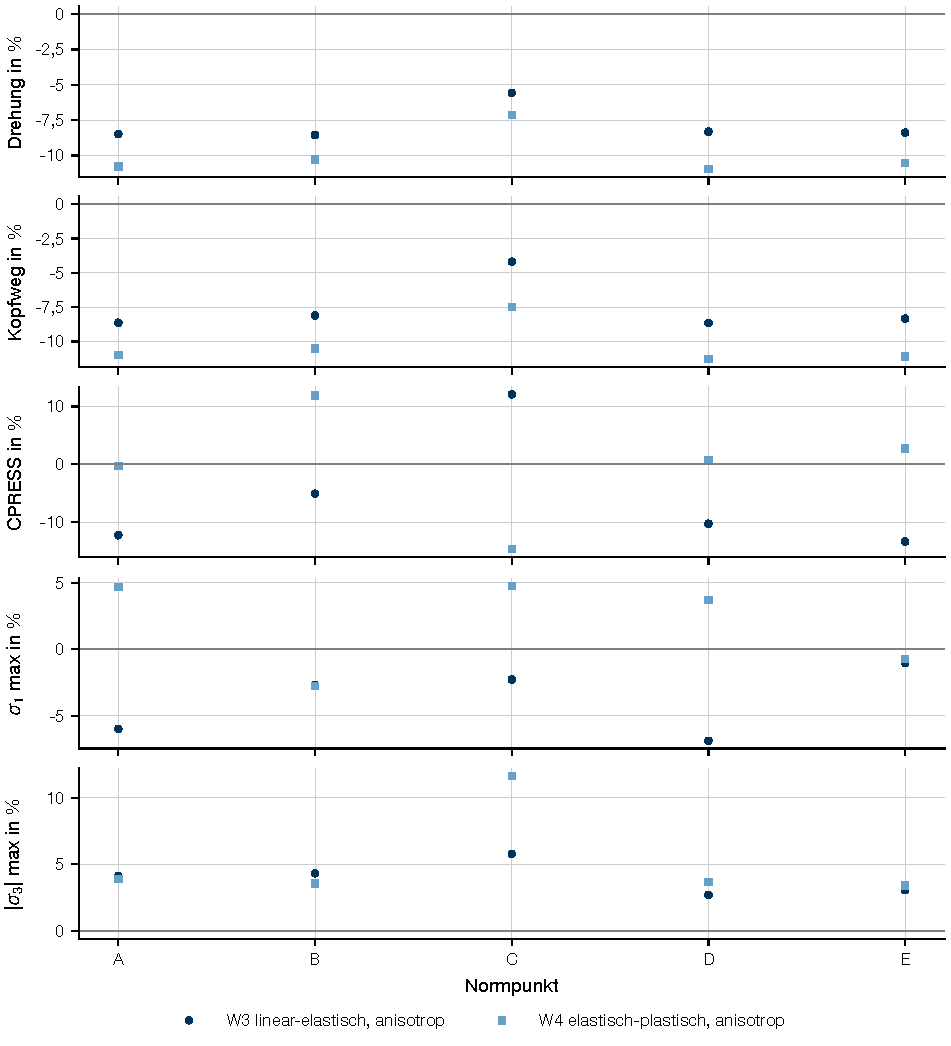
\includegraphics[width=\textwidth]{kap5/orientierungseffekt_16nm_qs}
    \caption{Orientierungseffekt, relative Änderung jeder Größe, wenn an die Stelle des CONVERSE-Mappings die CT-Zonen des Berichts treten, bei gleichem Netz und gleicher Karte an den Normpunkten A bis E. Die Legende nennt die Werkstoffstufe, für die der Tausch gerechnet ist (W3 und W4), $16$\,Nm, quasistatisch. Größtwerte über die Zahnbreite, Marker ohne Linie, weil der Verlauf zwischen den Punkten nicht gerechnet ist.}
    \label{fig:orientierungseffekt_16nm_qs}
\end{figure}

% Herkunft:
% Absatz 1 (Auswertung): ADR-119 Decision 1 bis 3 (architecture_decisions.md ab Zeile 2858); FVA856-I.txt Kapitel 6.2
%   und 6.3 (Bild 15 bis 18 S. 17 bis 19, Bild 23 S. 24, Gl. (1) S. 17 AI); 80_output/fe/faserorientierung/bericht.md
%   Kopf (Zonen, Streifen 0,20/0,40 mm, 13320 Elemente).
% Absatz 2 und Tabelle: bericht.md Abschnitt 1 (Zonen gegen CT) und 3 (Drittel): LT 0,63/0,71, LF 0,34/0,86, LFU
%   0,35/0,83, LFO 0,62/0,76, S 0,41/0,55, LÜU 0,28/0,76, LÜM 0,20/0,70, LÜO 0,25/0,60, M 0,30/0,35, U 0,67/0,70;
%   rechte Zonen RF 0,33, RFU 0,39, RFO 0,70, RT 0,61 (Differenz ≤ 0,08); a11 Mittel 0,55 bis 0,66; Drittel AI
%   mitte: LT 0,64, LF 0,68, LFU 0,71, LFO 0,75, S 0,35, LÜU 0,59, LÜM 0,54, LÜO 0,52, M 0,39, U 0,69; λ3 mitte
%   gegen außen −8 bis −27 % (LT −10, LFU −8, S −14, RFU −11, RF −12, RT −27, LÜM −8, RÜO −21, RÜM −10, RÜU −13,
%   U −10); Neigung z−/z+: LF 31,9/−50,8, LFU 45,8/−50,8, LFO 71,7/−64,5, LÜU 30,1/−42,1, LÜM 41,6/−47,7, RFU
%   45,9/−45,3 → "25 bis 75" und "45 bis 69" (ADR-119 Findings). Richtungen: Abschnitt 2 (LT −79,2, RT 81,6, LF
%   −39,6, RF 49,9, LÜU −48,1, LÜM −15,1, LÜO −46,9, LFU/LFO/S/RFO axial mit Anteil 0,05 bis 0,45, M −42,7, U
%   89,4; Bild 18: −81,6/84,4, −27,5/28,5, ∓32,5, −12,8/−18,5/−89,1, −85,3).
% Absatz 4 (Richtung, Ursache, Empfindlichkeit): ADR-119 Findings und Consequences (virtueller Verteiler 238 Punkte
%   r 15,0 bis 19,1 mm in der Stegebene, Füllung von z = 0 zu beiden Stirnseiten; Band 0,1/0,3 mm: ≤ 0,04, obere
%   Flanken/Kopf ≤ 0,13, Übergangszonen ≤ 0,5; Schliffbild offen, FIB-03).
% Absatz 5 (Vollrad): 80_output/fe/faserorientierung_vollrad/ring/bericht.md (LF 0,12 bis 0,53, LFO 0,23 bis 0,75,
%   RFO 0,24 bis 0,79; Zahn 27 = Zahn 3); ADR-119 Amendment 2026-10-13 (Wellen von 12 bis 15 Zähnen, Zonenmittel
%   innerhalb 0,02 beim Taschenkörper; Wahl des Zahns als Eingabe).
% Absatz 6 (2 × 2-Schema): 80_output/fe/kst_e/vergleich_orientierung_AtoE/analyse.md (Drehung −4,8 bis −12,7 %,
%   Kopfverschiebung −3,0 bis −13,2 %, σ1 −7,6 bis +5,3 %, |σ3| +1,4 bis +12,1 %, Kontaktdruck A/D/E bis −18,8 %,
%   C +4 bis +18,5 %, W4 16 Nm C −14,7/−18,8 %); vergleich_orientierung_tab4_AtoE/analyse.md (W3: Drehung −6,8 bis
%   −12,0, σ1 −14,0 bis +3,3, |σ3| +0,6 bis +14,7 %); ADR-119 Amendment 2026-10-13 (DY1 größter, QS kleinster
%   Effekt; Größenordnung des Körpereffekts, kleiner als die Werkstoffstufe); Konsequenz für W3/W4: ADR-119
%   Consequences, ADR-116 Punkt 47 (b).
% Bildwunsch: kap5/faserorientierung_schnitt (fe/faserorientierung/schnitt_T3.svg), faserorientierung_zonen
%   (zonen_T3.svg, in bilder.yaml), faserorientierung_drittel (drittel_T3.svg), orientierungseffekt_16nm_qs
%   (fe/kst_e/vergleich_orientierung_AtoE/orientierungseffekt_LOAD_16NM_QS.svg); faserorientierung_vergleich
%   (vergleich_T3.svg) steht in bilder.yaml, wird hier durch die Tabelle ersetzt.
% Bibwunsch: FVA856-I vorhanden.
% Nomenklatur: AI, lambda_min/lambda_max (2.2) vorhanden; lambda_1 bis lambda_3 und a_11 (Orientierungsgrad,
%   größter Eigenwert des Elementtensors) prüfen.
% Offen: Schliffbild; Anspritzung des Berichtsrades; die Nachtlauf-Varianten mit Tabelle 4 sind nur für W3 gerechnet.

\section{Beanspruchung über dem Wälzweg}
\label{sec:waelzweg}

Die Serie aus \secref{sec:fe_modell} umfasst je Werkstoffstufe 99 Stellungen über $3{,}2$ Teilungen bei $8$, $12$ und $16$\,Nm auf dem Taschenkörper nach Zeichnung, der nach \secref{sec:stufen_raten_koerper} das Modell des realen Teils ist. Von den 396 Rechnungen liefen 387 vollständig. Fünf Stellungen von W1 und vier von W3 brachen im Schritt $16$\,Nm im Kantenkontakt mit flatternden Kontaktknoten auf den Radien $25{,}80$ und $25{,}90$\,mm ab (\secref{sec:kopfkante}) und fehlen in ihren Kurven bei $16$\,Nm. Die Ringserie der Voruntersuchungen lief mit 395 von 396 Rechnungen durch. Ihre Werte stehen zum Vergleich in \anhref{sec:anhang_f}. \figref{fig:vergleich_stufen_16nm} zeigt für $16$\,Nm den Verdrehwinkel des Ritzels, die Kopfverschiebung, den größten Kontaktdruck und die Fußspannungen $\sigma_{\mathrm{1}}$ und $|\sigma_{\mathrm{3}}|$ für W1 bis W4. Alle Werte sind Größtwerte über die Zahnbreite. \figref{fig:vergleich_stufen_8nm} zeigt dasselbe für $8$\,Nm. \tabref{tab:waelzweg_normpunkte} nennt die Werte an den Normpunkten A bis E und die Maxima mit ihrem Ort.

\begin{figure}[htbp]
	\centering
	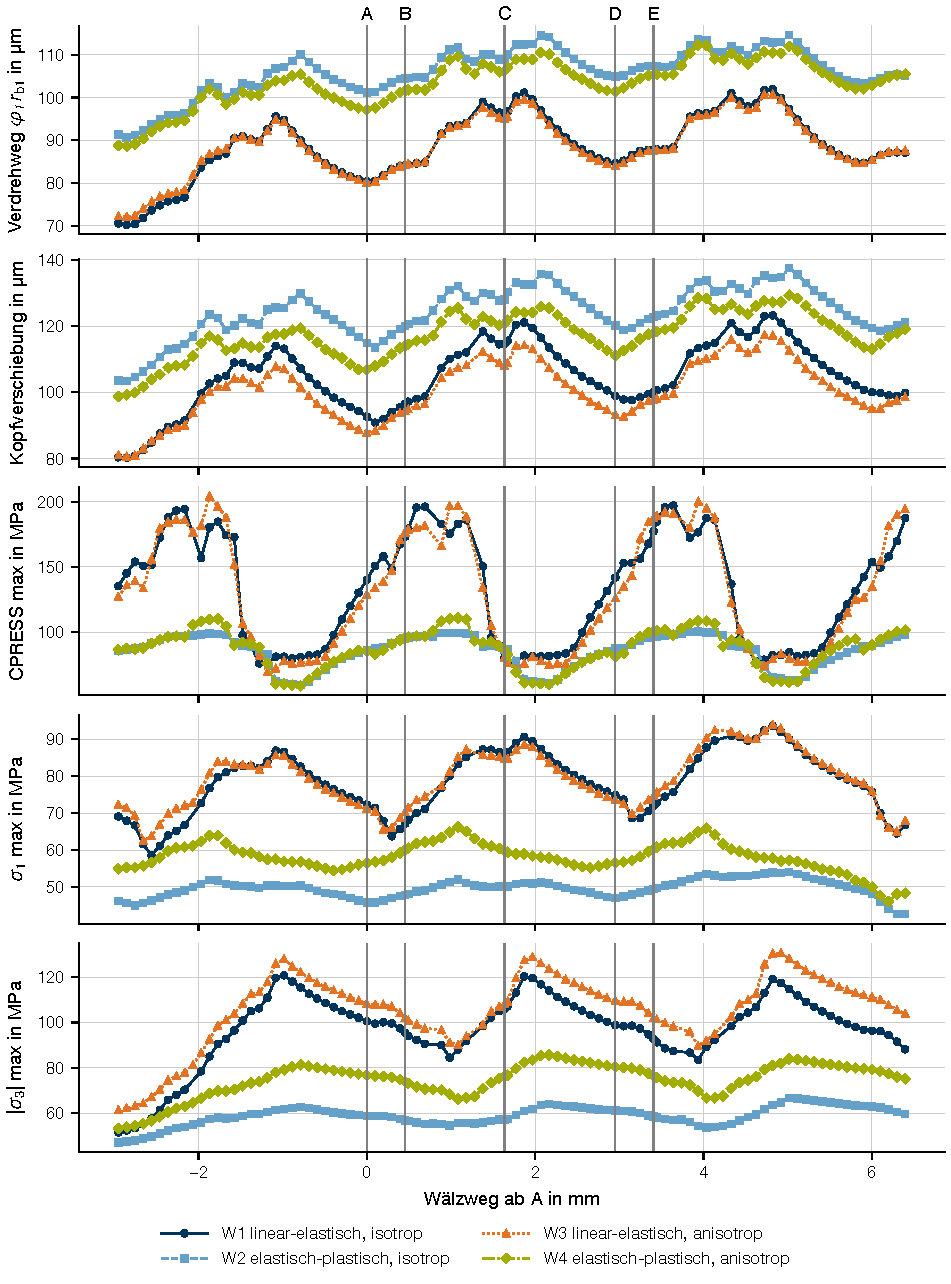
\includegraphics[width=\textwidth]{kap5/vergleich_stufen_16nm}
	\caption{Werkstoffstufen W1 bis W4 über dem Wälzweg bei $16$\,Nm, Taschenkörper, Kopfkante $r = 0{,}10$\,mm, quasistatisch: Verdrehwinkel, Kopfverschiebung, größter Kontaktdruck und die Fußspannungen $\sigma_{\mathrm{1}}$ und $|\sigma_{\mathrm{3}}|$ als Größtwerte über die Zahnbreite. Senkrechte Linien markieren die Normpunkte A bis E.}
	\label{fig:vergleich_stufen_16nm}
\end{figure}

\begin{figure}[htbp]
	\centering
	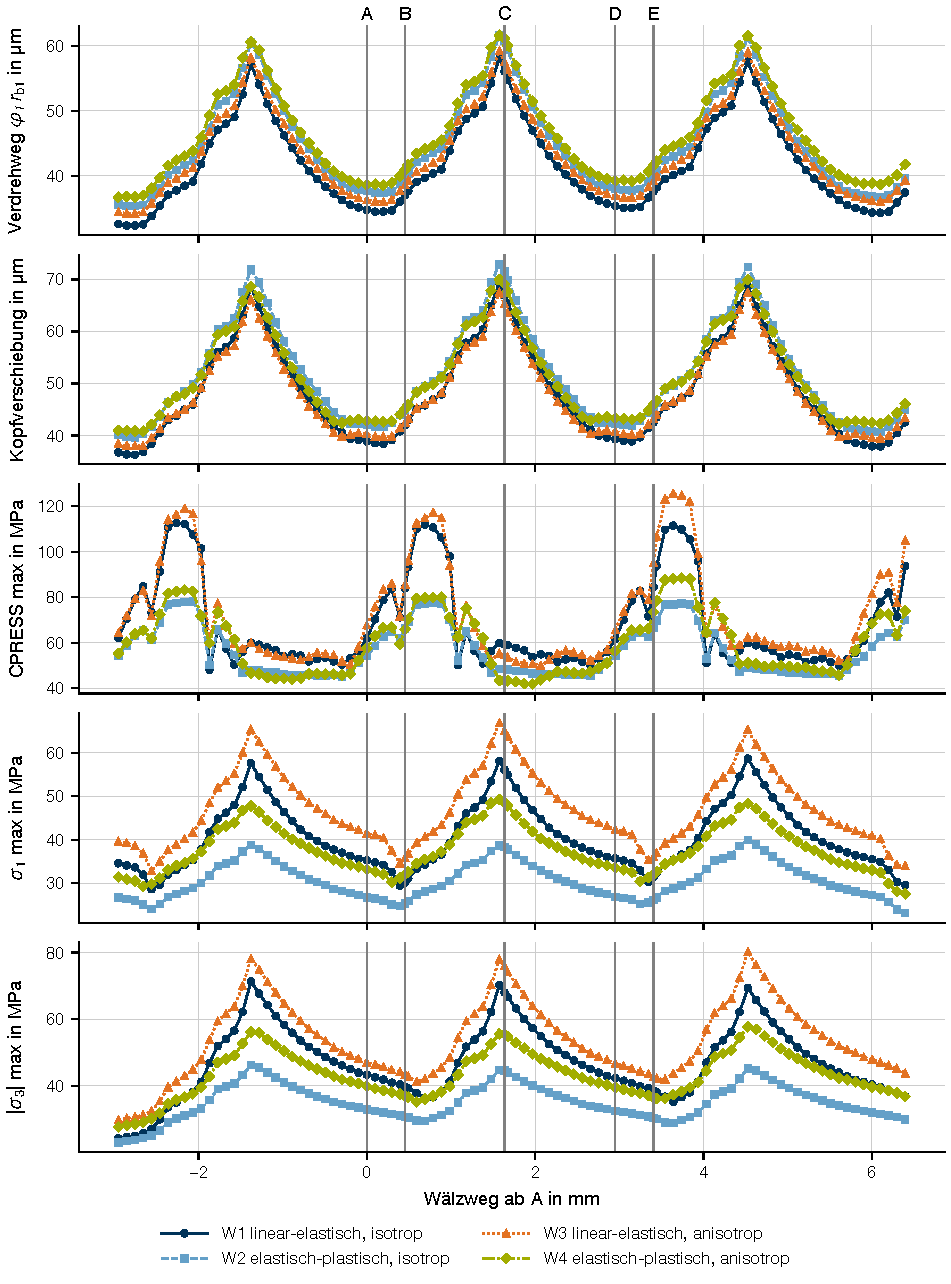
\includegraphics[width=\textwidth]{kap5/vergleich_stufen_8nm}
	\caption{Werkstoffstufen W1 bis W4 über dem Wälzweg bei $8$\,Nm, Taschenkörper, Kopfkante $r = 0{,}10$\,mm, quasistatisch. Größen wie in \figref{fig:vergleich_stufen_16nm}, die Achsen je Bild skaliert.}
	\label{fig:vergleich_stufen_8nm}
\end{figure}

\begin{table}[htbp]
	\caption{Beanspruchung an den Normpunkten A, C und E und Maximum über den Wälzweg je Werkstoffstufe, Taschenkörper, quasistatische Karte, Größtwerte über die Zahnbreite: größte Zugspannung $\sigma_{\mathrm{1}}$ und größte Druckspannung $|\sigma_{\mathrm{3}}|$ der Fußrundung in MPa, Verdrehwinkel des Ritzels $\varphi_{\mathrm{1}}$ in mrad an C und größter Kontaktdruck $p_{\mathrm{max}}$ in MPa über dem Wälzweg.}
	\label{tab:waelzweg_normpunkte}
	\centering
	\footnotesize
	\setlength{\tabcolsep}{4pt}
	\begin{tabular}{L{1.0cm}L{0.8cm}L{1.0cm}L{1.0cm}L{1.0cm}L{1.1cm}L{1.0cm}L{1.0cm}L{1.0cm}L{1.1cm}L{1.1cm}L{1.1cm}}
		$T_{2}$  & Stufe & $\sigma_{\mathrm{1}}$ A & $\sigma_{\mathrm{1}}$ C & $\sigma_{\mathrm{1}}$ E & $\sigma_{\mathrm{1}}$ max & $|\sigma_{\mathrm{3}}|$ A & $|\sigma_{\mathrm{3}}|$ C & $|\sigma_{\mathrm{3}}|$ E & $|\sigma_{\mathrm{3}}|$ max & $\varphi_{\mathrm{1}}$ C & $p_{\mathrm{max}}$ \\
		\hline
		\arrayrulecolor{black!30}
		$8$\,Nm  & W1    & $36{,}6$                & $59{,}4$                & $36{,}5$                & $61{,}4$                  & $50{,}7$                  & $75{,}1$                  & $46{,}5$                  & $75{,}1$                    & $2{,}70$                 & $124{,}6$          \\
		\hline
		         & W2    & $27{,}8$                & $38{,}8$                & $29{,}3$                & $40{,}8$                  & $37{,}0$                  & $45{,}8$                  & $35{,}1$                  & $47{,}1$                    & $2{,}81$                 & $80{,}3$           \\
		\hline
		         & W3    & $35{,}8$                & $57{,}6$                & $37{,}9$                & $61{,}5$                  & $54{,}4$                  & $77{,}8$                  & $51{,}3$                  & $80{,}2$                    & $2{,}66$                 & $121{,}2$          \\
		\hline
		         & W4    & $29{,}4$                & $44{,}3$                & $32{,}4$                & $46{,}3$                  & $45{,}1$                  & $58{,}5$                  & $43{,}7$                  & $59{,}1$                    & $2{,}76$                 & $83{,}6$           \\
		\hline
		$12$\,Nm & W1    & $54{,}4$                & $72{,}7$                & $54{,}2$                & $76{,}8$                  & $75{,}5$                  & $90{,}4$                  & $70{,}0$                  & $96{,}3$                    & $3{,}35$                 & $161{,}4$          \\
		\hline
		         & W2    & $37{,}7$                & $44{,}4$                & $40{,}1$                & $48{,}1$                  & $49{,}4$                  & $51{,}4$                  & $47{,}7$                  & $58{,}1$                    & $3{,}60$                 & $95{,}9$           \\
		\hline
		         & W3    & $53{,}8$                & $71{,}0$                & $56{,}4$                & $77{,}7$                  & $81{,}5$                  & $92{,}9$                  & $76{,}9$                  & $104{,}2$                   & $3{,}31$                 & $158{,}0$          \\
		\hline
		         & W4    & $43{,}3$                & $52{,}0$                & $46{,}7$                & $55{,}9$                  & $62{,}5$                  & $67{,}0$                  & $61{,}6$                  & $75{,}2$                    & $3{,}53$                 & $103{,}3$          \\
		\hline
		$16$\,Nm & W1    & $72{,}3$                & $86{,}2$                & $72{,}0$                & $93{,}6$                  & $100{,}5$                 & $105{,}9$                 & $92{,}6$                  & $120{,}7$                   & $4{,}02$                 & $197{,}1$          \\
		\hline
		         & W2    & $45{,}8$                & $50{,}0$                & $49{,}4$                & $54{,}1$                  & $58{,}8$                  & $57{,}1$                  & $58{,}4$                  & $66{,}6$                    & $4{,}54$                 & $100{,}4$          \\
		\hline
		         & W3    & $71{,}3$                & $84{,}6$                & $74{,}8$                & $94{,}0$                  & $108{,}3$                 & $108{,}0$                 & $102{,}1$                 & $130{,}7$                   & $3{,}96$                 & $204{,}1$          \\
		\hline
		         & W4    & $56{,}5$                & $59{,}8$                & $60{,}3$                & $66{,}3$                  & $76{,}6$                  & $76{,}1$                  & $76{,}3$                  & $85{,}6$                    & $4{,}43$                 & $111{,}0$          \\
		\hline
		\arrayrulecolor{black}
	\end{tabular}
\end{table}

Die größte Zugspannung der Fußrundung erreichen die Stufen W1, W2 und W3 nicht an einem Normpunkt, sondern $1{,}1$ bis $1{,}6$\,mm hinter E im verlängerten Eingriff, wo die Ritzelkopfkante den Zahn trägt. Die plastische anisotrope Stufe W4 erreicht sie $0{,}2$ bis $0{,}6$\,mm vor C. Der mittlere Zahn trägt von $0{,}47$ bis $0{,}60$ Teilungen vor A bis $0{,}38$ bis $0{,}55$ Teilungen hinter E, bei den plastischen Stufen und bei $16$\,Nm am längsten. Der Einfluss der Kopfkantenrundung ist in \secref{sec:kopfkante} beziffert. Die Auflösung von 30 Stellungen je Teilung ist ausreichend. Mit 15 Stellungen ändern sich die Maxima um höchstens $2{,}4$\,\%, mit sechs um bis zu $13$\,\%.

Die Werkstoffstufen wirken in zwei Richtungen, auf dem Taschenkörper aber anders verteilt als auf dem Ring der Voruntersuchungen. Die Anisotropie der linearen Stufe ändert die Zugspannung an C um $-3$ bis $-2$\,\% und an B und E um $+4$ bis $+5$\,\%, die Druckspannung um $+2$ bis $+11$\,\%. Der Verdrehwinkel des Ritzels bleibt innerhalb von $1{,}5$\,\%. Auf dem Ring lag W3 an C noch $16$ bis $18$\,\% über W1 (\secref{sec:stufen_raten_koerper}). Der nachgiebige Steg des Taschenkörpers nimmt dem anisotropen Zahn an C einen Teil der Biegung ab. Die Plastizität senkt die Spannungen. Von W1 auf W2 fällt die Zugspannung an C um $35$, $39$ und $42$\,\% bei $8$, $12$ und $16$\,Nm, die Druckspannung um $39$ bis $46$\,\% und der größte Kontaktdruck um $35$ bis $49$\,\%. Der Verdrehwinkel des Ritzels wächst dabei um $4$ bis $13$\,\% an C und um bis zu $26$\,\% an A. Zwischen W3 und W4 wirkt die Plastizität mit $23$ bis $29$\,\% an C schwächer. Unter den plastischen Stufen bleibt die Anisotropie mit $+14$ bis $+20$\,\% in der Zugspannung an C und $+30$ bis $+33$\,\% in der Druckspannung erhalten, bei nahezu gleichem Verdrehwinkel des Ritzels. An C liegen damit W1 und W3 in den Spannungen nahezu gleich und über W4, W4 liegt über W2. In den Verformungen liegen W2 und W4 über W1 und W3.

% Herkunft:
% Absatz 1 (Serie, Abbruch): 80_output/fe/kst_e/series_20layers_bore33_round0p1f12_30perpitch_margin1_qs_gerechnet/
%   analyse/analyse.md Kopf und Abschnitt 1 (396 Stellungsdateien, 99 je Serie, pos_073_W1_QS abgebrochen bei
%   LOAD_16NM, flatternde Kontaktknoten, FE-19); Gitter 30 je Teilung, Rand 1,00 Teilungen, Wälzweg A bis E 3,406 mm,
%   Teilung 2,952 mm (Abschnitt 4).
% Tabelle: analyse.md Abschnitt 2 (8/12/16 Nm, Spalten A, C, E, Maximum; Verdrehwinkel an C; Kontaktdruck Maximum).
% Absatz 2 (Ort der Maxima, Eingriff, Kante, Auflösung): Abschnitt 2 (Ort ab A: σ1 W1/W2 4,533 bis 4,884 mm = 1,1 bis
%   1,5 mm hinter E = 3,406 mm; W3/W4 1,165 bis 1,882 mm nahe C = 1,703 mm); Abschnitt 4 (trägt ab −1,378 bis −1,771
%   = 0,47 bis 0,60 Teilungen vor A, bis 4,428 bis 4,822 = 0,35 bis 0,48 hinter E); Abschnitt 5 (Nebenzahn 168,3/
%   256,6/336,3 N gegen 162,4/243,6/322,2 N = +3,7/+5,3/+4,4 %; Maxima +0,1 bis +4,9 %; B und E σ1 −7,5/−4,7,
%   −8,3/−5,3, −8,7/−5,7 %, Kontaktdruck −9,9/−9,0, −10,8/−9,5, −9,1/−8,0 %); Abschnitt 6 (15 je Teilung ≤ 2,5 %,
%   6 je Teilung bis 14,7 %).
% Absatz 3 (Stufen): Abschnitt 3 (W1 → W3 σ1 A bis E +15,0 bis +19,9 %, |σ3| +8,5 bis +11,9 %, Drehung +1,6 bis
%   +4,7 %, Kontaktdruck C −7,7/−11,1/−11,5 %, E +12,3/+12,3/+14,5 %; W1 → W2 σ1 C −31,8/−37,9/−41,0 %, |σ3| C
%   −34,4/−41,1/−44,0 %, Kontaktdruck max −30,7/−38,3/−46,0 %, Drehung C +8,4/+8,4/+12,9 %, A +8,2/+16,0/+26,6 %;
%   W3 → W4 σ1 C −25,3/−30,5/−33,0 %; W2 → W4 σ1 +22,7 bis +34,8 %, Drehung −0,7 bis +4,0 %).
% Bildwunsch: kap5/vergleich_stufen_16nm und vergleich_stufen_8nm (analyse/vergleich_stufen_LOAD_16NM.svg,
%   vergleich_stufen_LOAD_8NM.svg); gleiche Skalierung beider Bilder prüfen (Hausregel).
% Bibwunsch: keiner.
% Nomenklatur: sigma_1, sigma_3 (vorhanden), varphi_1 (Verdrehwinkel des Ritzels, mrad; prüfen), p_max (größter
%   Kontaktdruck; prüfen).
% Offen: σ1-Karte; die Serien der Dehnratenkarten DY1/DY2 liegen nur an A bis E vor (4.3).

\section{Bemessung nach Stommel et al.}
\label{sec:stommel_ergebnis}

\subsection{Methode wie veröffentlicht}
\label{sec:stommel_veroeffentlicht}

Der Nachweis nach \secref{sec:auswertung_beanspruchung} wurde auf alle 99 Stellungen je Serie des Taschenkörpers aus \secref{sec:waelzweg} angewendet. Die Lastgeschichte jedes Knotens besteht aus dem unbelasteten Zustand und den vollständigen Stellungen eines Lastschritts. Eingestellt waren der Überlastungsfall F2, der zyklische Weg über die Hauptspannungen und die Abminderungsklasse teilkristallin verstärkt für das Verfahren wie veröffentlicht. Berichtet werden die beiden Fußrundungen des mittleren Zahns T3 mit 2562 Knoten. Die Randzähne tragen den Sektorrand. \tabref{tab:stommel_veroeffentlicht} nennt je Lastschritt den Knoten der größten zyklischen Auslastung $a_{\mathrm{B,V}}$ mit seiner statischen Auslastung $a_{\mathrm{stat}}$ und der vorhergesagten Lastwechselzahl auf der synthetischen Wöhlerlinie. W2 ist die Hauptlinie, W1 die lineare Referenz. Daneben steht die gemessene Lastwechselzahl der Bruchlinie. Sie ist keine Anrisslinie, der Vergleich ist deshalb einseitig und wird in \secref{sec:genauigkeit} in drei Stufen geführt.

\begin{table}[htbp]
    \caption{Nachweis nach Stommel et al. wie veröffentlicht an den Fußrundungen des Zahns T3, quasistatische Karte bei $80$\,\textdegree C, Überlastungsfall F2: kritischer Knoten mit Lage, zyklische Auslastung $a_{\mathrm{B,V}}$, statische Auslastung $a_{\mathrm{stat}}$ dort, Zahl der Fußknoten über $1$ und vorhergesagte Lastwechselzahl $N_{\mathrm{pred}}$. Daneben die gemessene Lastwechselzahl $N_{\mathrm{L},50\%}$ der Bruchlinie aus \secref{sec:woehlerlinien}.}
    \label{tab:stommel_veroeffentlicht}
    \centering
    \footnotesize
    \setlength{\tabcolsep}{4pt}
    \begin{tabular}{L{0.8cm}L{1.0cm}L{2.9cm}L{1.1cm}L{1.1cm}L{1.5cm}L{1.5cm}L{1.5cm}L{1.8cm}}
        Stufe & $T_{2}$ in Nm & kritischer Knoten        & $a_{\mathrm{B,V}}$ & $a_{\mathrm{stat}}$ & Fußknoten $a_{\mathrm{B,V}} > 1$ & Fußknoten $a_{\mathrm{stat}} > 1$ & $N_{\mathrm{pred}}$  & $N_{\mathrm{L},50\%}$ gemessen \\
        \hline
        \arrayrulecolor{black!30}
        W1    & $8$           & Fuß T2/T3, $z = 0{,}00$  & $1{,}72$           & $0{,}84$            & $1536$                           & $0$                               & $1{,}6 \cdot 10^{3}$ & $2{,}67 \cdot 10^{7}$          \\
        \hline
        W1    & $12$          & Fuß T3/T4, $z = 0{,}00$  & $2{,}69$           & $1{,}06$            & $2312$                           & $176$                             & sofort               & $5{,}96 \cdot 10^{6}$          \\
        \hline
        W1    & $16$          & Fuß T3/T4, $z = 0{,}00$  & $10{,}40$          & $1{,}64$            & $2486$                           & $944$                             & sofort               & $1{,}36 \cdot 10^{6}$          \\
        \hline
        W2    & $8$           & Fuß T3/T4, $z = -5{,}93$ & $1{,}30$           & $0{,}42$            & $905$                            & $0$                               & $1{,}7 \cdot 10^{5}$ & $2{,}67 \cdot 10^{7}$          \\
        \hline
        W2    & $12$          & Fuß T3/T4, $z = -5{,}93$ & $1{,}64$           & $0{,}52$            & $1943$                           & $0$                               & $4{,}3 \cdot 10^{3}$ & $5{,}96 \cdot 10^{6}$          \\
        \hline
        W2    & $16$          & Fuß T3/T4, $z = -5{,}93$ & $1{,}96$           & $0{,}66$            & $2228$                           & $0$                               & sofort               & $1{,}36 \cdot 10^{6}$          \\
        \hline
        \arrayrulecolor{black}
    \end{tabular}
\end{table}

% TK erledigt (nein, Bruchlinie; Vergleich einseitig in drei Stufen, Satz vor der Tabelle und in 7.1): Bei der Bruchlinie in Abschnitt 6.3 ist da auch tatsächlich mit den ersten Anrissen gerechnet? Sonst kann man schlecht gegen NL 50 % gemessen vergelichen, wenn das Buch und wir in der Erklärung sagen, dass das Verfahren auf ersten Anriss und nicht Bruchmechanik ausgelegt ist und jetzt aber verglichen wird mit der Buchlinie? 

Mit der plastischen isotropen Stufe W2 besteht der statische Nachweis an allen Fußknoten. Die zyklische Auslastung liegt bei $1{,}30$, $1{,}64$ und $1{,}96$. Die vorhergesagte Lastwechselzahl fällt mit dem Moment von $1{,}7 \cdot 10^{5}$ über $4{,}3 \cdot 10^{3}$ auf sofortiges Versagen bei $16$\,Nm, wo sie die Grenze von $10^{4}$ Lastspielen des Verfahrens unterschreitet. Die lineare Stufe W1 verletzt bei $12$ und $16$\,Nm an 176 und 944 Fußknoten den statischen Nachweis und sagt schon bei $8$\,Nm nur $1{,}6 \cdot 10^{3}$ Lastwechsel vorher. Der kritische Knoten von W2 liegt in der Fußrundung zwischen T3 und T4 nahe der Stirnseite bei $z = -5{,}93$\,mm von $\pm 7{,}5$\,mm. Er sitzt am Fuß der belasteten Flanke des Zahns T4 mit $h = 0{,}49$. Unter dem eigenen Zahn steht er im Zug, unter dem Nachbarzahn im Druck. Dass der Knoten zu T4 gehört, folgt aus seinem Winkel von $94{,}1$° um die Radachse, $2{,}9$° von der Zahnmitte T4 und $4{,}1$° von der Zahnmitte T3 entfernt. Dazu kommt die Kontaktspur des Modells, die auf der Flanke jedes Zahns zur Seite des kleineren Winkels liegt. Bei W1 liegt er in der Zahnmitte. Auf dem Ringkörper der Voruntersuchungen lag der kritische Knoten von W2 auf der Druckseite derselben Fußrundung mit $R \approx -0{,}4$ und einer Vorhersage von $3{,}5 \cdot 10^{5}$ bis $1{,}7 \cdot 10^{3}$ Lastwechseln. Der Steg des Taschenkörpers verschiebt die Lastgeschichte der Fußknoten so, dass die Zugseite maßgebend wird.

\begin{figure}[htbp]
    \centering
    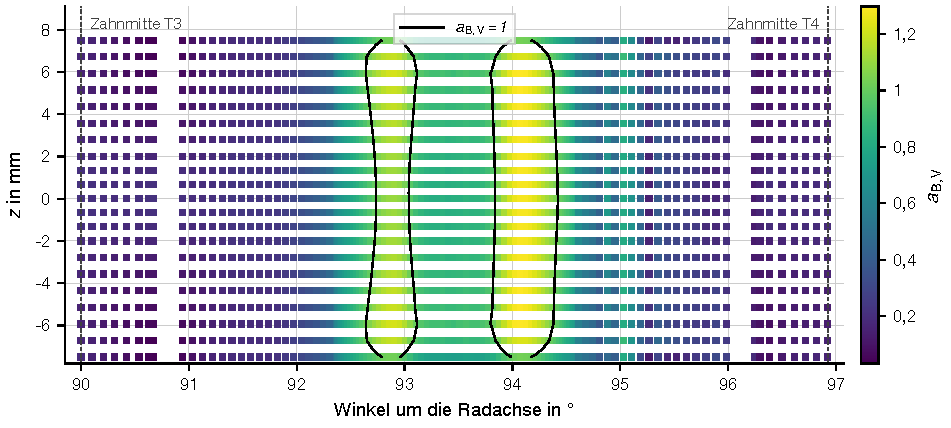
\includegraphics[width=\textwidth]{kap5/stommel_karte_8nm_w2}
    \caption{Zyklische Auslastung $a_{\mathrm{B,V}}$ über der Oberfläche zwischen den Mitten der Zähne T3 und T4, also über der Fußrundung, den beiden zugewandten Flanken und den Kopfflächen, Winkel um die Radachse über der Zahnbreite, W2 elastisch-plastisch isotrop, quasistatisch, $8$\,Nm. Der leere Streifen zwischen Kopffläche und Flanke bei $90{,}7$ bis $90{,}9$° und $96{,}0$ bis $96{,}2$° ist die Kopffase der STplus-Kontur, die das Netz mit einer Elementreihe ohne Zwischenknoten überspannt.}
    \label{fig:stommel_karte_8nm}
\end{figure}

% TK erledigt (Karte neu: Grid hinten, Zahnmitten T3/T4 als Linien, Grenzlinie a_B,V = 1 mit Legende, Ausschnitt auf die Zahnmitten; Schwarzweiß bleibt eine Farbkarte, die Grenzlinie trägt die Aussage): Schlecht, wenn schwarz weiß, hast dud a eine gute Idee? Wenn nicht, dann passt das schön, sieht gut aus. Aber Grid bitte auch weider in den Hintergrund und kannst du noch senksrechte Linien einfügen mit den Bezeichnungen T3 und T4, also direkt bei der mittleren Position des Zahnkopfes, also Zahnmitte? Dann kann man sich noch besser hineinversetzen, da der Leser erstmal an sich nicht weiß, wo jetzt der 0 Grad Zahn sein soll und den Winkel um die Radachse so nicht nullen kann im Kopf. Verstehst du?

\begin{figure}[htbp]
    \centering
    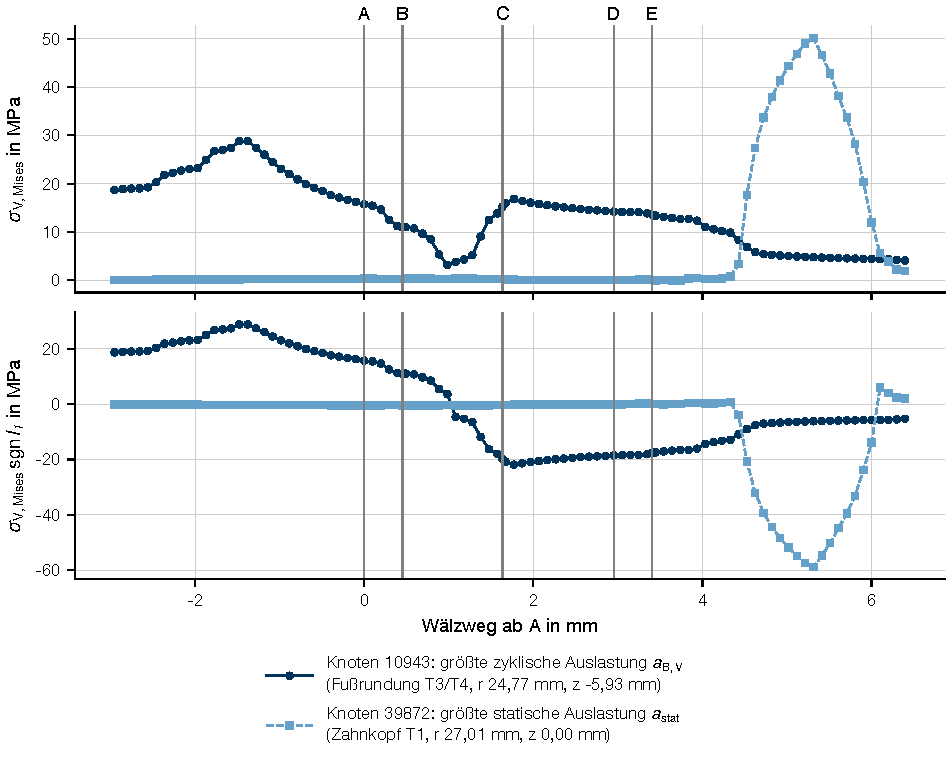
\includegraphics[width=\textwidth]{kap5/stommel_verlauf_8nm_w2}
    \caption{Vergleichsspannung $\sigma_{\mathrm{V}}$ und vorzeichenbehaftete von-Mises-Spannung der beiden kritischen Knoten der größten zyklischen und der größten statischen Auslastung über dem Wälzweg, W2, quasistatisch, $8$\,Nm. Senkrechte Linien an den Normpunkten A bis E.}
    \label{fig:stommel_verlauf_8nm}
\end{figure}

\figref{fig:stommel_karte_8nm} trägt die zyklische Auslastung von W2 bei $8$\,Nm über der Fußrundung zwischen T3 und T4 und über den angrenzenden Flanken bis zu den Zahnmitten auf. Die Auslastung über eins liegt in zwei Bändern entlang der Fußrundung, an 955 der 83\,650 Knoten. Das Band bei $94{,}1$° gehört zum Fuß der belasteten Flanke des Zahns T4. Es trägt den Größtwert $1{,}30$ in zwei stirnseitennahen Knoten bei $z = \pm 5{,}93$\,mm auf dem Radius $24{,}78$\,mm. Das Band bei $92{,}8$° gehört zum Fuß der unbelasteten Flanke des Zahns T3, der im Druck steht, solange T3 trägt, und in den Zug kommt, sobald T4 trägt. Im Band bei $94{,}1$° fällt die Auslastung zur Zahnmitte hin auf $1{,}29$, und die Linie $a_{\mathrm{B,V}} = 1$ schließt das Band gegen die Druckseite und gegen die Flanke ab. \figref{fig:stommel_verlauf_8nm} zeigt die Lastgeschichte der beiden kritischen Knoten über dem Wälzweg. Der Knoten der größten zyklischen Auslastung liegt in dieser Fußrundung. Er steht im Zug, solange der Zahn T4 trägt, mit $33$\,MPa Spitze, und wechselt in den Druck, sobald die Last auf den Nachbarzahn T3 übergeht. Daraus folgen die Amplitude $28{,}3$\,MPa und die Mittelspannung $4{,}6$\,MPa. Der Knoten der größten statischen Auslastung ist ein Kopfknoten des Zahns T1 mit $50$\,MPa Vergleichsspannung unter dem Kontakt des Ritzels. Seine Spannung tritt in einer Stellung auf und bleibt mit $0{,}77$ unter der statischen Grenze.

Gegen die Bruchlinie des Laufversuchs liegt die Vorhersage mit W2 bei $8$\,Nm um den Faktor $160$ und bei $12$\,Nm um den Faktor $1400$ zu niedrig, bei $16$\,Nm sagt sie sofortiges Versagen vorher. Das Verhältnis wächst mit dem Moment. Der Nachweis endet beim ersten makroskopischen Anriss, der Laufversuch beim Bruch. Die Anrissfenster aus \secref{sec:woehlerlinien} verkleinern den Abstand bei $8$\,Nm auf den Faktor $20$ bis $46$. Bei $12$ und $16$\,Nm wurden die ersten Anrisse nicht ausdrücklich dokumentiert, so dass dort nur eine obere Schranke bleibt und die Prüfanweisung in \chapref{chap:zusammenfassung} die Dokumentation der Anrisse für die folgenden Läufe verlangt. Die Einordnung dieser Abstände folgt in \secref{sec:genauigkeit}.

% TK erledigt (Satz zur fehlenden Dokumentation bei 12 und 16 Nm mit Verweis auf die Prüfanweisung): Ah, hier hast du es schon erklärt. Vielleicht noch darauf eingehen kurz, dass die Anrisse für 12 und 16 Nm leider nicht ausdrücklich dokumentiert wurden und dies für die folgenden Versuche zwingend dokumentiert werden sollte. sieeh ausblick oder wo du es eh schon dann mit erwähnt hast.

\subsection{Anisotrope Erweiterung}
\label{sec:stommel_anisotrop}

Für die anisotropen Stufen W3 und W4 wurde die Vergleichsspannung durch die Hill-Vergleichs\-spannung im Faserrahmen mit allen sechs Verhältnissen der Karte ersetzt, nach \secref{sec:auswertung_beanspruchung}. Die Orientierung ist in allen Nachweisen dieses Abschnitts die des CONVERSE-Mappings, nicht die der CT-Zonen. Die Abminderungsfaktoren nehmen die Klasse teilkristallin unverstärkt, weil die Karte an Zugversuchen des verstärkten Werkstoffs kalibriert ist und die Klasse der verstärkten Werkstoffe die Querschwäche ein zweites Mal zählen würde. \tabref{tab:stommel_hill} nennt die Ergebnisse an den Fußrundungen des Zahns T3 auf dem Taschenkörper, dazu W1 unter Hill als Methodenvergleich mit denselben Spannungen wie in \tabref{tab:stommel_veroeffentlicht}.

\begin{table}[htbp]
    \caption{Nachweis mit der Hill-Vergleichs\-spannung im Faserrahmen an den Fußrundungen des Zahns T3, Klasse teilkristallin unverstärkt, quasistatisch, Überlastungsfall F2: kritischer Knoten, zyklische und statische Auslastung, Fußknoten über $1$. $\infty$ bedeutet eine Vergleichsspannung jenseits des Endes der Isotherme bei $80$\,\textdegree C.}
    \label{tab:stommel_hill}
    \centering
    \footnotesize
    \setlength{\tabcolsep}{4pt}
    \begin{tabular}{L{1.6cm}L{1.2cm}L{3.2cm}L{1.3cm}L{1.3cm}L{1.8cm}L{1.8cm}L{1.6cm}}
        Stufe   & $T_{2}$ in Nm & kritischer Knoten        & $a_{\mathrm{B,V}}$ & $a_{\mathrm{stat}}$ & Fußknoten $a_{\mathrm{B,V}} > 1$ & Fußknoten $a_{\mathrm{stat}} > 1$ & $N_{\mathrm{pred}}$ \\
        \hline
        \arrayrulecolor{black!30}
        W3 Hill & $8$           & Fuß T3/T4, $z = -0{,}67$ & $3{,}25$           & $\infty$            & $2390$                           & $54$                              & sofort              \\
        \hline
        W3 Hill & $12$          & Fuß T3/T4, $z = 1{,}33$  & $4{,}67$           & $\infty$            & $2505$                           & $614$                             & sofort              \\
        \hline
        W3 Hill & $16$          & Fuß T3/T4, $z = 1{,}33$  & $55{,}1$           & $\infty$            & $2544$                           & $1116$                            & sofort              \\
        \hline
        W4 Hill & $8$           & Fuß T2/T3, $z = 2{,}79$  & $2{,}45$           & $0{,}45$            & $2128$                           & $0$                               & sofort              \\
        \hline
        W4 Hill & $12$          & Fuß T2/T3, $z = 2{,}79$  & $3{,}01$           & $0{,}66$            & $2411$                           & $0$                               & sofort              \\
        \hline
        W4 Hill & $16$          & Fuß T2/T3, $z = 2{,}79$  & $3{,}55$           & $\infty$            & $2498$                           & $9$                               & sofort              \\
        \hline
        W1 Hill & $8$           & Fuß T2/T3, $z = 0{,}67$  & $3{,}29$           & $\infty$            & $2271$                           & $112$                             & sofort              \\
        \hline
        W1 Hill & $12$          & Fuß T3/T4, $z = 2{,}00$  & $5{,}68$           & $\infty$            & $2467$                           & $588$                             & sofort              \\
        \hline
        W1 Hill & $16$          & Fuß T3/T4, $z = -2{,}79$ & $\infty$           & $\infty$            & $2546$                           & $1049$                            & sofort              \\
        \hline
        \arrayrulecolor{black}
    \end{tabular}
\end{table}

Unter Hill wandert der kritische Knoten von der Stirnseite in die Zahnmitte, bei W3 nach $z = -0{,}7$ und $1{,}3$\,mm, bei W4 nach $2{,}8$\,mm und bei W1 nach $0{,}7$ bis $2{,}8$\,mm. Dort liegen nach \secref{sec:faserorientierung} die Fasern der Flankenzonen axial, die Biegespannung in der Stirnebene wirkt quer zur Faser, und die Karte schwächt diese Richtung. An der Stirnseite folgen die Fasern der Kontur und tragen die Biegung in Faserrichtung. Dass der kritische Knoten ohne Hill nahe der Stirnseite liegt, hat seinen Grund im Spannungszustand. An der freien Stirnfläche verschwindet die Spannung normal zur Stirnseite. Der zweiachsige Zustand liefert bei ähnlicher größter Hauptspannung eine höhere von-Mises-Spannung und einen kleineren Mehraxialitätsgrad als der dreiachsige Zustand in der Zahnmitte, in dem die Querdehnung behindert ist. Die Hill-Vergleichs\-spannung liegt an den Fußknoten deutlich über der von-Mises-Spannung. Die Fließspannungsverhältnisse der Karte betragen im Mittel über die Knoten $R_{11} = 0{,}88$, $R_{22} = 0{,}69$, $R_{33} = 0{,}57$, $R_{12} = 0{,}58$, $R_{13} = 0{,}54$ und $R_{23} = 0{,}46$, so dass die Schubspannung im Faserrahmen fast doppelt gewichtet wird. Bei W3 und bei W1 unter Hill überschreitet die Vergleichsspannung an 54 bis 1116 Fußknoten das Ende der Isotherme, so dass dort keine Dehnung abgelesen werden kann und der statische Nachweis entfällt. Die plastische anisotrope Stufe W4 besteht den statischen Nachweis bis $12$\,Nm, bei $16$\,Nm liegen neun Fußknoten jenseits der Isotherme. Zyklisch liegt sie mit $2{,}5$ bis $3{,}5$ um den Faktor $1{,}8$ über W2. \figref{fig:stommel_verlauf_16nm_w4} zeigt den Verlauf der Hill-Vergleichsspannung der beiden über das ganze Rad kritischen Knoten von W4 bei $16$\,Nm, der Knoten der größten zyklischen und der größten statischen Auslastung. Dazu ist die vorzeichenbehaftete von-Mises-Spannung mit dem Vorzeichen der betragsgrößten Hauptspannung aufgetragen. Beide sind Kopfknoten unter dem Ritzelkontakt an den Stirnseiten der Zähne T1 und T5, nicht die Fußknoten der Tabelle, die der Nachweis unter Hill jenseits der Isotherme findet. Der Knoten der größten statischen Auslastung liegt auf der Druckseite, seine Kurve ist deshalb negativ. Die Höhe der Auslastung hängt an der Klasse der Abminderungsfaktoren, die das Buch für einen Werkstoff mit aufgelöster Richtungsabhängigkeit nicht festlegt. Mit der Klasse der verstärkten Werkstoffe läge sie noch höher. Belastbar sind damit zunächst die Lage des kritischen Knotens und der Vergleich der Stufen. Um die Erweiterung auch für die Lebensdauer zu kalibrieren, braucht es die Orte der ersten Anrisse über der Zahnbreite aus den Laufversuchen. Die Prüfanweisung in \chapref{chap:zusammenfassung} verlangt sie.

% TK erledigt (Kurven im Text erklärt: Hill-Vergleichsspannung beider kritischer Knoten plus vorzeichenbehaftete von-Mises-Spannung, Druckknoten negativ; letzter Satz auf die Kalibrierung über die Anrissorte gerichtet): Also bild 5.9 ist für mich noch nicht eindeutig, vorallem die Bezeichnungen Vergelichsspannung und hill. Mises ist doch die vergelichsspannung im normalfall oder nicht? Und warum ist die eine so positiv und die andere so negativ? Und der letzte Satz passt auch nicht in die Richtung, die ich untersuche. Mit dem Satz würde ich so hinnehmen, dass das Verfahren nicht für die Lebensdauer verwendbar ist, aber genau das versuchen wir ja hinzubekommen und jetzt ist ja eh noch mit faktoren gerechnet, die noch nie für sowas angewendet wurden. Aber da bräuchte es mehr Versuchsdaten, um die Anrisse besser zu lokalisieren und auf Faktoren zurückzuschließen oder?


% TK erledigt (Stirnseite: ebener Spannungszustand, höhere von-Mises-Spannung und kleineres h; Mitte unter Hill: Fasern axial, Biegung quer zur Faser): Warum ist ohne Hill überhaupt der höchste Auslastungsgrad eher bei der Stirnseite, das kann ich mir nicht wirklich erklären, sind die Effekte da durch Mehraxialität und anderen Einflüssen auf den dynamischen Auslastungsgrad so prägsam, dass die größeren Spannungen in der Zahnmitte trotzdem nicht so relevant sind? Bitte mal erklären, warum sich das dann unter Hill auch so verschiebt. Achso, bei Hill, da die mittlere Zone die schwächste ist. Ok, aber warum dann bei mises eher Stirnseite, das checke ich noch nicht?

\begin{figure}[htbp]
    \centering
    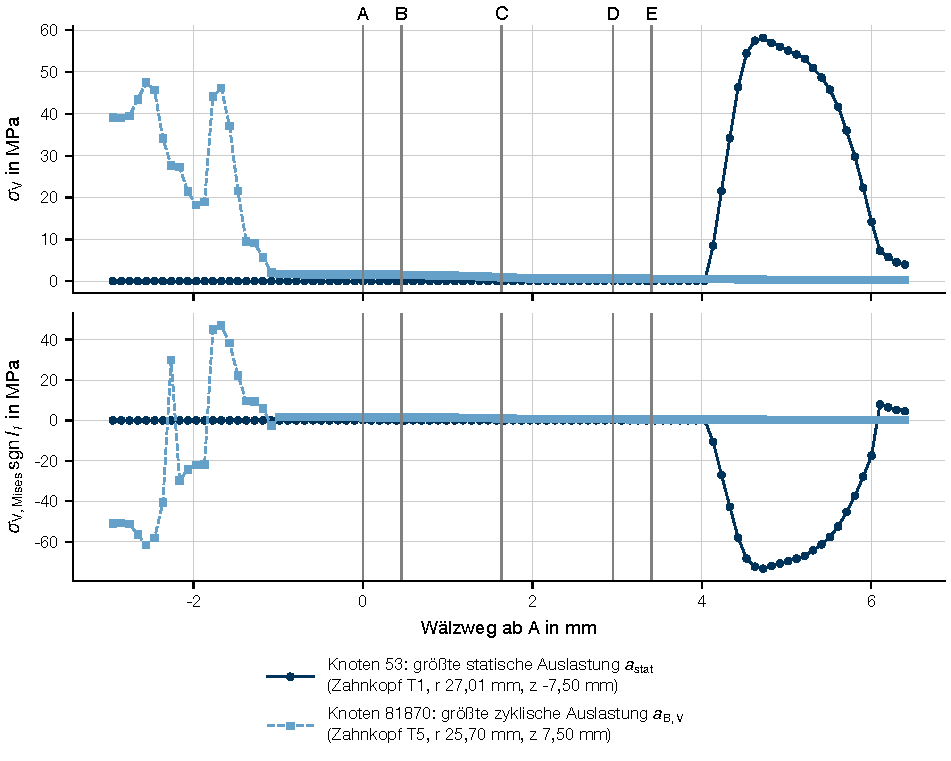
\includegraphics[width=\textwidth]{kap5/stommel_verlauf_16nm_w4hill}
    \caption{Hill-Vergleichs\-spannung und vorzeichenbehaftete von-Mises-Spannung der beiden über das ganze Rad kritischen Knoten (größte zyklische und größte statische Auslastung, beide Kopfknoten unter dem Ritzelkontakt) über dem Wälzweg, W4 elastisch-plastisch anisotrop, Taschenkörper, quasistatisch, $16$\,Nm. Senkrechte Linien an den Normpunkten A bis E.}
    \label{fig:stommel_verlauf_16nm_w4}
\end{figure}

\subsection{Globalmaxima, Überlastungsfälle und Vergleich mit S-Life Plastics}
\label{sec:stommel_global_slife}

Über alle 83\,650 Knoten des Rades liegt die größte Auslastung bei W2 in der Fußrundung selbst, mit $1{,}96$ bei $16$\,Nm. Die Kopfknoten der Zähne auf dem Radius $25{,}80$\,mm, wo die gerundete Ritzelkopfkante die Radflanke belastet, folgen mit $1{,}93$ am Kopf von T2 dicht dahinter. Bei W1 geht $a_{\mathrm{B,V}}$ an diesen Kopfknoten gegen unendlich. Unter Hill kommt die erste Knotenreihe unter dieser Spur auf $25{,}78$\,mm hinzu, mit Vergleichsspannungen jenseits der Isotherme. Die Kopfknoten sind Kontaktspannungszustände und keine Aussage zur Zahnfußermüdung. Die Tabellen dieses Abschnitts beziehen sich deshalb auf die Fußrundungen des Zahns T3 und nennen das Globalmaximum daneben. Im Versuch ist genau diese Spur der Ort der Einarbeitung der Ritzelkopfkante und bei $16$\,Nm von vier Flankenbrüchen an drei Rädern (\secref{sec:schadensbilder}). Der Überlastungsfall F2 ist nach \secref{sec:auswertung_beanspruchung} der Lastpfad des Rades mit konstantem Spannungsverhältnis $R$ an jedem Knoten. Die plastischen Stufen weichen von der Proportionalität zwischen Moment und Spannung leicht ab.

% TK erledigt (Schadensbilder in 6.2 aufgenommen und hier sowie in 7.2 mit der Kantenspur verknüpft; 5.3 rechnet mit des CONVERSE-Mappings, so im Text benannt): Da wäre jetzt doch interessant, mal die Schadensbilder 70_input\71_Messungen\Mikroskop\Bilder\Schadensbilder_Kunststoffraeder\8Nm\F4092_1_Lw_170824_202610.jpg 70_input\71_Messungen\Mikroskop\Bilder\Schadensbilder_Kunststoffraeder\12Nm\F4092_1_Lw_170817_202610.jpg 70_input\71_Messungen\Mikroskop\Bilder\Schadensbilder_Kunststoffraeder\16Nm\F4092_1_Lw_170820_202610.jpg zu analysieren, da das genau der Bereich sein könnte, in dem sich das Phänomen auch bei den realen Laufrädern ereignet und sich die Ritzelkopfkante in das Kunststoffrad einarbeitet. Was schon top wäre für die Auswertung. Ist 5.3.3 schon mit dem CT Orientierungsprofil oder dem eigenen Spritzgegossenem? Aber das ist natürlich interessant. Bitte da nochmal reinblicken und das dann mit aufnehmen in den späteren Auswertungskapiteln.

Als Gegenprobe wurde die Stellung C mit W1 in S-Life Plastics mit den Einstellungen nach \secref{sec:auswertung_beanspruchung} ausgewertet, rein schwellend mit $R = 0$, die Spannungen ungemittelt als Elementknotenwert eines Elements, die kritische Ebene mit $11{,}25$° Schritt. Verglichen wurden vier Knoten, zwei Zugknoten der Fußrundung in Zahnmitte und nahe der Stirnseite, ein Druckknoten der gegenüberliegenden Fußrundung und ein Kopfknoten. \tabref{tab:slife_vergleich} nennt die Werte bei $16$\,Nm. Die Hauptspannungen stimmen bis auf die Mittelung überein, mit $82{,}84$ gegen $82{,}85$\,MPa am Zugknoten der Zahnmitte und bis $5$\,\% am Kopfknoten. Der statische Nachweis stimmt auf $5$\,\%. Die verbleibende Differenz stammt aus der Dehnung, die S-Life auf seiner angepassten Isotherme liest, $2{,}49$ gegen $2{,}62$\,\% der interpolierten Punkte der Karte. Am Kopfknoten unter Druck mit $h = -1{,}3$ gibt S-Life $1{,}01$ gegen $0{,}42$ des eigenen Nachweises, der die Druckhauptspannungen nach Gleichung (6.17) durch $1{,}3$ teilt und die zulässige Dehnung bei $h = -1{,}3$ liest. S-Life wendet dort ein anderes Kriterium an. Im zyklischen Nachweis sind Amplitude, Wechselfestigkeit und Mittelspannungsfaktor gleich, mit $41{,}41$ gegen $41{,}42$\,MPa, $20{,}12$ gegen $20{,}19$\,MPa und $0{,}82$ gegen $0{,}815$. Der einzige Unterschied ist die statische Kappe der zulässigen Amplitude. Die beiden Lesarten unterscheiden sich in der Größe, von der die Mittelspannung abgezogen wird. S-Life nimmt die statische Zulässigkeit des unbelasteten Extremzustands von $47{,}32$\,MPa, also die zulässige Spannung der Isotherme ohne Rücksicht auf den Spannungszustand des Knotens, und erhält am Zugknoten $5{,}91$\,MPa. Der eigene Nachweis nimmt die statische Bauteilfestigkeit $\sigma_{\mathrm{stat}}(h)$ des maßgebenden Zustands, die das Buch im statischen Nachweis mit dem Mehraxialitätsgrad des Knotens liest, und erhält $13{,}27$\,MPa. Daraus folgen $a_{\mathrm{B,V}}$ von $6{,}53$ gegen $2{,}67$. Auf der Druckseite übersteigt die Mittelspannung von $49{,}6$\,MPa die Kappe von S-Life, so dass dessen Auslastung ins Unendliche läuft, während der eigene Nachweis $10$\,MPa behält. Die Umsetzung ist damit in Spannungen, statischem Nachweis, Amplitude und Festigkeit bestätigt. Der Unterschied in der Kappe ist benannt und reproduzierbar. Das Buch legt die Lesart in den Gleichungen (6.24) bis (6.26) \cite[S.~374]{Sto18} nicht eindeutig fest. Einen Maßstab für die Genauigkeit nennt es an anderer Stelle, und zwar für den Vergleich mit dem Versuch, nicht für den Unterschied zweier Lesarten. Für die Ermüdungsfestigkeit gilt eine Abweichung der berechneten von der gemessenen Lastspielzahl um den Faktor zwei bis drei als gut und das Treffen der Größenordnung als angemessen \cite[S.~375]{Sto18}. An diesem Maßstab gemessen liegt die vorhergesagte Lastwechselzahl der eigenen Lesart nach \tabref{tab:stommel_veroeffentlicht} bei $8$ und $12$\,Nm zwei bis drei Größenordnungen unter der Bruchlinie, also außerhalb des Bandes. Die Lesart von S-Life mit der kleineren Kappe läge noch weiter darunter. Der Unterschied der Lesarten, Faktor $2{,}5$ in der Auslastung und über die Neigung $k$ von rund $15$ mehrere Größenordnungen in der Lastspielzahl, ändert an dieser Einordnung nichts, bleibt aber als Unterschied benannt. Die Arbeit führt deshalb den eigenen Nachweis als wörtliche Lesart des Buches und S-Life als Referenzimplementierung nebeneinander, ohne eine der beiden auszuschließen.
% TK erledigt (Lesart der Kappe im Text erklärt, S-Life gegen eigene Lesart, Einordnung über die Genauigkeitsaussage des Buchs S. 375 wie vom Nutzer zitiert): Meinst du, welches der sigma a,i ... was du für den Nachweis verwendet hast und was die verwenden? Aber in der folgenden Seite steht auch: "Speziell für den Bereich der Ermüdungsfestigkeit ... Faktoren von 2 bis 3 ... als gut zu bezeichnen sind." Also können

\begin{table}[htbp]
    \caption{S-Life Plastics 4.0.0 gegen den eigenen Nachweis an vier Knoten der Stellung C, W1, quasistatische Karte, $16$\,Nm. Je Zelle erster Wert S-Life, zweiter Wert eigener Nachweis: größte Hauptspannung, statische Auslastung, Amplitude, Wechselfestigkeit, angewandte zulässige Amplitude und zyklische Auslastung. S-Life mit ungemittelten Elementwerten, eigener Nachweis mit gemittelten Elementknotenwerten.}
    \label{tab:slife_vergleich}
    \centering
    \footnotesize
    \setlength{\tabcolsep}{4pt}
    \begin{tabular}{L{2.6cm}L{1.9cm}L{1.6cm}L{1.9cm}L{1.8cm}L{2.0cm}L{1.6cm}}
        Knoten                      & $\sigma_{\mathrm{1}}$ bzw. $\sigma_{\mathrm{3}}$ in MPa & $a_{\mathrm{stat}}$ & $\sigma_{\mathrm{a}}$ in MPa & $\sigma_{\mathrm{W}}$ in MPa & $\sigma_{\mathrm{B}}$ angewandt in MPa & $a_{\mathrm{B,V}}$  \\
        (S-Life / eigener Nachweis) &                                                         &                     &                              &                              &                                        &                     \\
        \hline
        \arrayrulecolor{black!30}
        Zug, Zahnmitte              & $82{,}84$ / $82{,}85$                                   & $1{,}39$ / $1{,}45$ & $41{,}41$ / $41{,}42$        & $20{,}12$ / $20{,}19$        & $5{,}91$ / $13{,}27$                   & $6{,}53$ / $2{,}67$ \\
        \hline
        Zug, nahe Stirnseite        & $84{,}19$ / $81{,}67$                                   & $1{,}42$ / $1{,}49$ & $42{,}06$ / $40{,}84$        & $20{,}12$ / $20{,}19$        & $5{,}26$ / $14{,}80$                   & $7{,}52$ / $2{,}42$ \\
        \hline
        Druck, Fußrundung           & $-99{,}12$ / $-99{,}17$                                 & $1{,}08$ / $1{,}11$ & -- / $3{,}62$                & $20{,}12$ / $20{,}19$        & $0$ / $26{,}12$                        & $\infty$ / $4{,}60$ \\
        \hline
        Kopf                        & $-79{,}88$ / $-76{,}29$                                 & $1{,}01$ / $0{,}42$ & -- / $14{,}47$               & $20{,}12$ / $20{,}19$        & -- / $26{,}12$                         & $4{,}23$ / $1{,}07$ \\
        \hline
        \arrayrulecolor{black}
    \end{tabular}
\end{table}

% TK erledigt (Bildunterschrift und Kopfzeile nennen die Reihenfolge S-Life / eigener Nachweis): Also bei der Tabelle 5.5 sollte schon erkennbar sein auf den ersten Blick, was eigenes verfahern und S-Life ist. Man kann es sich mit dem Text deuten, aber die Tabelle sollete auch für sich alleine sprechen. Noch in der Tabellen beschriftung aufnehmen, erster wert, zweiter wert oder innerhalb der Tabelle anders kennzeichen.s

% Herkunft:
% 5.3.1: analyse.md Abschnitt 7 (Tabelle je Serie: W1 8/12/16 Nm 1,63/2,03/4,47, a_stat 0,81/0,94/1,31, Knoten > 1
%   1438/2295/2479 und 0/256/920, N 3,91e3/0/0, kritische Knoten 13999 (T2_T3, z −5,25), 5817 (T3_T4, z −6,75);
%   W2 1,24/1,47/1,74, 0,48/0,58/0,68, 660/1489/2097, 0/0/0, 3,54e5/2,24e4/1,65e3, Knoten 10852/10853 (T3_T4,
%   z −6,00)); ADR-118 Amendment 2026-10-12 Punkt 2 (Einstellungen: F2, Hauptspannungsroute, Klasse verstärkt),
%   Punkt 4 (Druckseite, R < 0, z −6,0 bis −6,75), Amendment 2026-10-13 (R ≈ −0,4: +32/−14 MPa bei 8 Nm);
%   N_L,50 % aus 80_output/messungen/woehler/woehler.md (2,671e7, 5,964e6, 1,357e6); Faktoren 2,671e7/3,54e5 =
%   75, 5,964e6/2,24e4 = 266, 1,357e6/1,65e3 = 822; Anrissfenster 8 Nm: 3,22e6/3,54e5 = 9,1 bis 7,66e6/3,54e5
%   = 21,6 (kst-E_69), 3,65e6/3,54e5 = 10,3 bis 6,61e6/3,54e5 = 18,7 (kst-E_75).
% 5.3.2: analyse.md Abschnitt 7 (W3 Hill 3,12/3,85/10,38 mit ∞, Knoten 37549 (T2_T3, z −0,75), 21518 (T3_T4, z
%   −3,75), > 1: 2326/2518/2560 und 74/530/1138; W4 Hill 2,16/2,58/3,03, 0,44/0,53/0,73, 54026 (z 2,25), 26552
%   (z −3,00), 1954/2358/2495 und 0/0/4, N 1,22e3/0/0; W1 Hill 3,07/3,96/16,64 mit ∞, 2173/2469/2543 und
%   79/570/1054); ADR-118 Amendment E7 (σ_Hill = 1,74 σ_Mises im Median an C, σ_13 ≈ 37 MPa mit R_13 0,53; Klasse
%   teilkristallin unverstärkt, kein doppeltes Zählen, Buch S. 346); W4 gegen W2: 2,16/1,24 = 1,74, 2,58/1,47 =
%   1,76, 3,03/1,74 = 1,74.
% 5.3.3: ADR-118 Amendment 2026-10-12 Punkt 3 (Kopfknoten r 25,80, a_B,V → ∞ für W1, W2 16 Nm 1,84 T2 head;
%   Hill: Knotenreihe r 25,78, σ_V 93 bis 105 MPa; FE-22), Amendment 2026-10-13 (Überlastfall als Lastpfad, F2,
%   E2 offen); S-Life: 80_output/fe/kst_e/frozen_mesh_20layers_bore33_gerechnet/stommel/vergleich_slife.md 16 Nm
%   (41472: 82,84/82,85, a_SK 1,388/1,452, σ_a 41,41/41,42, σ_WK 20,12/20,19, Kappe 5,91/13,27, a_BK 6,53/2,671;
%   6147: 84,19/81,67, 1,420/1,489, 42,06/40,84, 5,26/14,80, 7,52/2,416; 41143: −99,12/−99,17, 1,079/1,114, σ_a
%   eigen 3,62, Kappe 0 → a_BK 49 641 (als ∞ geschrieben), eigen 26,12/4,602; 5741: −79,88/−76,29, 1,010/0,425,
%   14,47, 26,12, 4,23/1,066); ADR-118 Amendment 2026-10-14 Findings 1 bis 4 (Dehnung 2,49 gegen 2,62 %, K_AK 0,82
%   gegen K_M 0,815, Kappe σ_S,allow,min 47,32 MPa, Gl. (6.17) Faktor 1,3, Lesart Gl. (6.24) bis (6.26) S. 365 bis
%   367 offen, Option cap = min_state).
% Bildwunsch: kap5/stommel_karte_8nm_w2 (stommel_W2_QS/karte_LOAD_8NM_T3_T4.svg), stommel_verlauf_8nm_w2
%   (stommel_W2_QS/verlauf_LOAD_8NM.svg), stommel_verlauf_16nm_w4hill (stommel_hill_W4_QS/verlauf_LOAD_16NM.svg).
% Bibwunsch: Sto18 vorhanden (Gl. (6.17), (6.24) bis (6.26)).
% Nomenklatur: a_B_V, a_stat, N_pred (prüfen: N_pred als vorhergesagte Lastwechselzahl, neu), sigma_a, sigma_W,
%   sigma_B, h, R, R_13 (Hill-Verhältnis, prüfen), sigma_stat, sigma_V vorhanden (3.7).
% Offen: Klassenwahl unter Hill; Überlastungsfälle F1 bis F4 (E2); Lesart der Kappe; die 12-Nm-Knotentabelle des
%   eigenen Nachweises fehlt in der S-Life-Datei (nur Spannungen).

\section{Einfluss der Zahnfußgeometrie}
\label{sec:fussgeometrie}

Die drei Fußrundungsformen aus \secref{sec:werkzeugkette} wurden mit den Parametern ihrer Quellen und mit den Optima der ebenen Parameterstudie am Rad gerechnet. Jede Variante ersetzt die Trochoide der Erzeugung zwischen dem Übergangsdurchmesser und der Lückenmitte. Netzvorlage, Ritzelfläche, Lastschritte und Stellungen bleiben die der Taschen-Grundlinie aus \secref{sec:fe_modell}. Gerechnet wurden die Werkstoffstufen W1 bis W4 mit den Dehnratenkarten QS, DY1 und DY2 an den Normpunkten A bis E, je Variante 60 Rechnungen. Alle sechs Varianten liegen vollständig vor.

\tabref{tab:fussrundung_konturen} stellt die Konturen nebeneinander. Die Ellipse nach Frühe \cite{Frue12} beginnt am Fußformkreis und legt den Fußkreis um $0{,}57$\,mm tiefer als die Trochoide. Ihr kleinster Krümmungsradius liegt bei $0{,}083$\,mm in der Lückenmitte. Die beiden Patentkonturen setzen am mittleren Durchmesser zwischen Nutzkreis und Fußformkreis an und füllen den Fuß bis auf $50{,}2$\,mm und $50{,}1$\,mm auf. Dadurch rückt der kleinste Abstand der Ritzelkopfkante zur Fußrundung von $0{,}49$\,mm auf $0{,}20$\,mm. Der Vorauswahl diente eine ebene Parameterstudie am Einzahnsektor mit dem eigenen Löser. Sie trägt das ganze Moment auf einem Zahn mit einem Lastfleck am Normpunkt B und liefert ein relatives Maß (\secref{sec:werkzeugkette}).

% TK erledigt (eigener Löser in 3.6 beschrieben: ebener Dehnungszustand, CPE4/CPE4I-Formulierungen, Abgleich mit Abaqus): Mir ist gerade aufgefallen, das noch an keiner Stelle eine Aussage zum eigenen FE Löser gesagt wurde. Wie der aufgebaut ist oder welche Einschränkungen der hat. Das wäre ja wie ein eigenes Abaqus oder wie kann ich mir das vorstellen, darüber hatten wir auch noch nicht gesprochen und du hast den einfach implementiert auf welcher Basis aber?

\begin{table}[htbp]
	\caption{Fußrundungsvarianten am Rad kst-E: Kennwerte der Konturen und Änderung der größten Zugspannung gegen die Trochoide nach der ebenen Parameterstudie (W1, $16$\,Nm, Lastfleck an B).}
	\label{tab:fussrundung_konturen}
	\centering
	\footnotesize
	\setlength{\tabcolsep}{4pt}
	\begin{tabular}{L{3.0cm}L{2.9cm}lllll}
		Kontur                  & Parameter                                        & Übergang   & Fußkreis   & $\rho_{\mathrm{min}}$ & Abstand Kopfkante & eben      \\
		                        &                                                  & mm         & mm         & mm                    & mm                &           \\
		\hline
		\arrayrulecolor{black!30}
		Trochoide der Erzeugung & $\rho_{\mathrm{aP0}}$                            & $50{,}157$ & $49{,}524$ & $0{,}240$             & $0{,}490$         & $0$       \\
		\hline
		Ellipse nach Frühe      & $\gamma$ $30$°, $a/b$ $3{,}0$                    & $50{,}157$ & $48{,}951$ & $0{,}083$             & $0{,}491$         & $-13$\,\% \\
		\hline
		Ellipse, Optimum        & $\gamma$ $25$°, $a/b$ $2{,}0$                    & $50{,}157$ & $49{,}041$ & $0{,}170$             & $0{,}491$         & $-25$\,\% \\
		\hline
		Bézier nach Patent      & $f$ $1{,}0$                                      & $51{,}210$ & $50{,}215$ & $0{,}633$             & $0{,}203$         & $-32$\,\% \\
		\hline
		Bézier, Optimum         & $f$ $2{,}5$                                      & $51{,}210$ & $49{,}796$ & $0{,}366$             & $0{,}203$         & $-35$\,\% \\
		\hline
		Bionisch nach Patent    & $\varphi$ $24{,}1$°, $r$ $0{,}3\,S_{\mathrm{L}}$ & $51{,}210$ & $50{,}124$ & $0{,}382$             & $0{,}203$         & $-32$\,\% \\
		\hline
		Bionisch, Optimum       & $\varphi$ $35$°, $r$ $0{,}2\,S_{\mathrm{L}}$     & $51{,}210$ & $49{,}811$ & $0{,}255$             & $0{,}203$         & $-38$\,\% \\
		\hline
		\arrayrulecolor{black}
	\end{tabular}
\end{table}

% TK (folgt mit Paket E10: Eingriffsstellung C der drei eigenen Optima als Bilder pair_mesh in den Anhang): vielleicht kann man da auch nochmal jeweils Plots der Eingriffsstellung der unterschiedlichen Geometrien (die eigenen optimierten reichen) in den Anhang mit aufnhemn.

\subsection{Zugspannung im Zahnfuß}
\label{sec:fussgeometrie_sigma1}

\begin{table}[htbp]
	\caption{Änderung der größten Zugspannung $\sigma_{\mathrm{1}}$ und des Verdrehwinkels des Ritzels gegen die Trochoide am Normpunkt C, $16$\,Nm, quasistatische Karte, je Werkstoffstufe.}
	\label{tab:fussrundung_sigma1_c}
	\centering
	\begin{tabular}{llllll}
		Kontur               & W1            & W2            & W3            & W4            & Verdrehwinkel W1 \\
		\hline
		\arrayrulecolor{black!30}
		Ellipse nach Frühe   & $-15{,}9$\,\% & $-6{,}0$\,\%  & $-4{,}3$\,\%  & $-7{,}8$\,\%  & $+6{,}3$\,\%  \\
		\hline
		Ellipse, Optimum     & $-24{,}4$\,\% & $-13{,}4$\,\% & $-15{,}0$\,\% & $-12{,}3$\,\% & $+5{,}4$\,\%  \\
		\hline
		Bézier nach Patent   & $-25{,}2$\,\% & $-15{,}7$\,\% & $-25{,}0$\,\% & $-17{,}2$\,\% & $-11{,}0$\,\% \\
		\hline
		Bézier, Optimum      & $-27{,}6$\,\% & $-20{,}5$\,\% & $-29{,}1$\,\% & $-25{,}4$\,\% & $-5{,}4$\,\%  \\
		\hline
		Bionisch nach Patent & $-27{,}4$\,\% & $-15{,}7$\,\% & $-26{,}2$\,\% & $-19{,}0$\,\% & $-10{,}2$\,\% \\
		\hline
		Bionisch, Optimum    & $-25{,}4$\,\% & $-15{,}8$\,\% & $-22{,}6$\,\% & $-21{,}2$\,\% & $-6{,}4$\,\%  \\
		\hline
		\arrayrulecolor{black}
	\end{tabular}
\end{table}

\figref{fig:fusseffekt_sigma1_16nm_qs} zeigt die relative Änderung der größten Zugspannung $\sigma_{\mathrm{1}}$ der Fußrundung gegen die Trochoide an den fünf Normpunkten bei $16$\,Nm und quasistatischer Karte, je ein Feld für W1 bis W4. Alle Werte sind Größtwerte über die Zahnbreite. Zwischen den Punkten ist der Verlauf nicht gerechnet, deshalb stehen Marker ohne Linie. \tabref{tab:fussrundung_sigma1_c} nennt die Zahlen am Normpunkt C, an dem die Grundlinie ihre größte Fußspannung erreicht.

\begin{figure}[htbp]
	\centering
	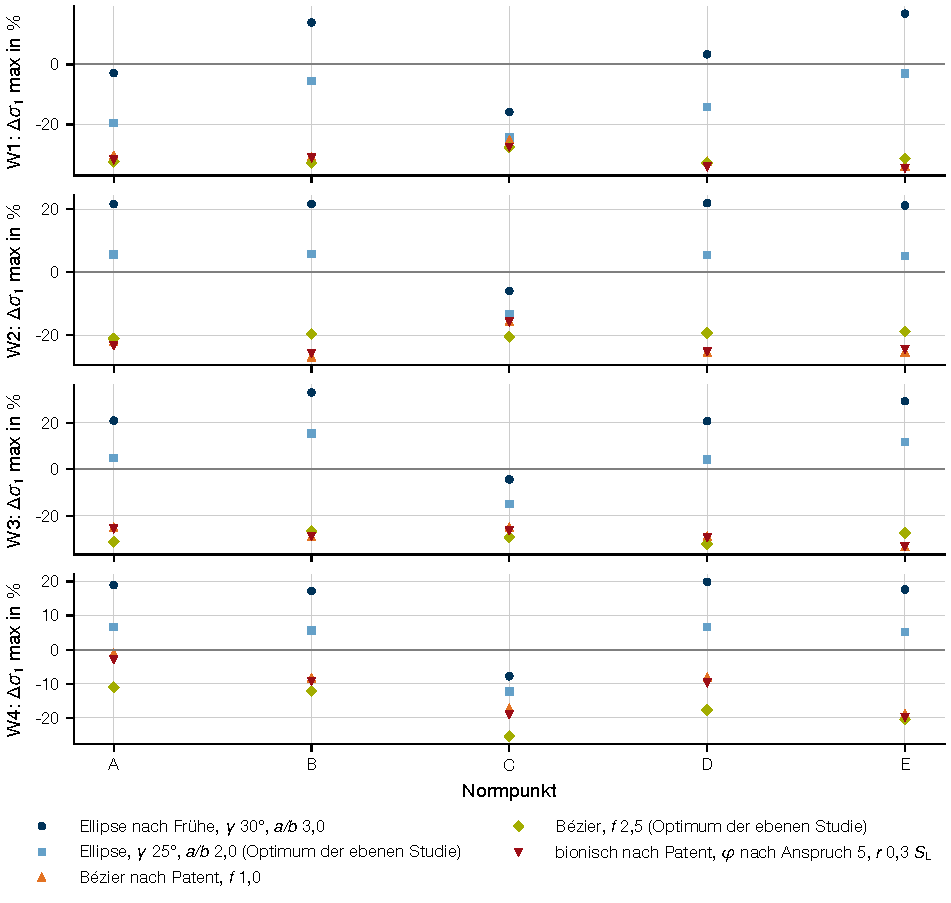
\includegraphics[width=0.95\textwidth]{kap5/fusseffekt_sigma1_16nm_qs}
	\caption{Fußrundungsvarianten gegen die Trochoide der Erzeugung: relative Änderung der größten Zugspannung $\sigma_{\mathrm{1}}$ an den Normpunkten A bis E je Werkstoffstufe (W1 bis W4 von oben nach unten), Taschenkörper, $16$\,Nm, quasistatische Karte. Größtwerte über die Zahnbreite, Marker ohne Linie.}
	\label{fig:fusseffekt_sigma1_16nm_qs}
\end{figure}

% TK (ja, bleibt das Ziel; Paket E10: Zwillinge für 8 und 12 Nm der Bilder aus Kapitel 5 in den Anhang F): Und allgemein für alle Grafiken, nimmst du dann in den anhang auch jeweils die nicht eingebundenen Zwillinge anderer Drehmomentstufen oder ... auf, die in den Haupttext einfach zu überflutend wären, aber trotzdem natürlich relevante INformationen enthalten? Ist das noch das Ziel für den Anhang?

Im räumlichen Modell bleibt die Reihenfolge der ebenen Studie im Wesentlichen erhalten, die Beträge am Normpunkt C fallen kleiner aus. Unter W1 sinkt die größte Zugspannung bei der Ellipse nach Frühe um $16$\,\% und beim Optimum der Ellipse um $24$\,\%. Die Bézierkonturen erreichen $25$\,\% und $28$\,\%, die bionische Kontur nach den Patentwerten $27$\,\% und das bionische Optimum der ebenen Studie $25$\,\%. Am Normpunkt B, an dem das ebene Modell belastet war, treffen die beiden Patentkonturen nach den Literaturwerten und das Bézier-Optimum den Wert der ebenen Studie auf drei Prozentpunkte. Das bionische Optimum verfehlt ihn. Die ebene Studie sagte ihm mit $38$\,\% die größte Minderung voraus, im räumlichen Modell bleiben an B $24$\,\% und an C $25$\,\%, so dass es hinter die Bézierkontur mit $f = 2{,}5$ zurückfällt. Die ebene Studie mit einem Lastfleck an B überzeichnet den Nutzen des flachen Fußes, weil sie die Lastaufteilung und den Kontakt nicht kennt. Die Ellipsen weichen an B ab, weil ihr Größtwert nicht auf dem Flankenteil der Fußrundung liegt, sondern in der Lückenmitte.

An allen fünf Normpunkten senken die Patentkonturen die Zugspannung. Unter W1 liegen die Änderungen zwischen $-20$\,\% und $-35$\,\%, unter W3 zwischen $-17$\,\% und $-33$\,\%. Das bionische Optimum mit seinem kleinen Radius liegt am unteren Ende dieser Spannen. Die Druckspannung $\sigma_{\mathrm{3}}$ der gegenüberliegenden Fußrundung fällt um bis zu $44$\,\%. Der aufgefüllte Fuß macht den Zahn steifer. Der Verdrehwinkel des Ritzels nimmt um $4$\,\% bis $22$\,\% ab, die Kopfverschiebung um bis zu $26$\,\%. Dadurch drückt die Kante des Ritzelkopfes an den Normpunkten B und E stärker auf die Flanke des Rades. Der größte Kontaktdruck steigt dort bei den Patentwerten um $21$\,\% bis $30$\,\%, bei den Optima der ebenen Studie um bis zu $53$\,\% (Bézier $f = 2{,}5$ und bionisch $\varphi = 35$°). Die Flankenpressung unter der Ritzelkopfkante ist nach \secref{sec:waelzweg} schon bei der Trochoide die höchste Beanspruchung des Rades und nach \secref{sec:schadensbilder} der Ort der Einarbeitung im Versuch. Jede Fußrundung, die den Fuß auffüllt, entlastet den Fuß und belastet die Flanke, so dass der Nutzen am Fuß mit einer höheren Pressung an der Kante erkauft wird.

Anders verhalten sich die Ellipsen. Am Normpunkt C sinkt die Zugspannung. An den Doppeleingriffspunkten A, B, D und E steigt sie bei der Ellipse nach Frühe um bis zu $17$\,\% unter W1, $22$\,\% unter W2, $33$\,\% unter W3 und $20$\,\% unter W4. Die Druckspannung wächst dort um bis zu $30$\,\% unter W1 und W2 und um bis zu $51$\,\% unter W3. Beim Optimum der Ellipse bleiben die Änderungen an diesen Punkten unter W1 negativ. Unter W2 bis W4 erreichen sie bis zu $+6$\,\%, $+15$\,\% und $+7$\,\%. In beiden Fällen sitzt der Größtwert in der Lückenmitte auf dem kleinsten Krümmungsradius der Kontur, bei der Trochoide dagegen auf dem Flankenteil der Fußrundung. Der Radius von $0{,}083$\,mm liegt unter der Auflösung der Netzvorlage, so dass die Zahlen der Ellipsen an der Lückenmitte netzbegrenzt sind. Die Reihenfolge gegenüber den Patentkonturen bleibt davon unberührt. Mit dem tieferen Fuß wird der Zahn nachgiebiger, der Verdrehwinkel des Ritzels wächst um $5$\,\% bis $11$\,\%.

% TK erledigt (Satz zur Flankenpressung als Grenze im Absatz darüber, Aufnahme in 7.3): Kommt dann irgendwo in der Auswertung auch ein Satz dazu, dass eh schon die Flankenpressung sehr sehr hoch ist und limitierend und eine Optimierung des Fußes die Flanke noch mehr beansprucht. Das ist ja mehr oder weniger auch das Ergebnis dieser Fußoptimierungsfestellung, richtig? Ich schreibe es nur hier schonmal mit hin, dass ich es nicht vergesse, mit aufzunehmen.

\subsection{Werkstoffstufen, Dehnraten und Last}
\label{sec:fussgeometrie_stufen}

\figref{fig:fusseffekt_raten_16nm} ordnet die Änderung am Normpunkt C je Variante, Werkstoffstufe und Dehnratenkarte. Die Plastizität der isotropen Karte halbiert den Nutzen der Varianten. Unter W2 bleiben von den $25$\,\% bis $28$\,\% der Patentkonturen $16$\,\% bis $21$\,\%. Unter den anisotropen Stufen W3 und W4 bleibt ein Nutzen von $4$\,\% bis $29$\,\% erhalten, bei der Ellipse nach Frühe wächst er von W3 zu W4 sogar. Die Dehnrate verschiebt die Änderungen bei den Patentkonturen nach den Literaturwerten um höchstens zwei Prozentpunkte. Bei den Ellipsen und beim bionischen Optimum unter W3 nehmen die Minderungen von QS zu DY2 um vier bis sechs Prozentpunkte ab, weil die steifere Karte die Lastaufteilung zum Nachbarzahn verschiebt. Mit der Last nimmt der Nutzen der Patentkonturen nach den Literaturwerten ab. Die Bézierkontur mindert die Zugspannung unter W1 bei $8$\,Nm um $32$\,\% und bei $16$\,Nm um $25$\,\%, die bionische Kontur um $33$\,\% und $27$\,\%. Das bionische Optimum bleibt unter W1 bei $25$\,\% auf allen drei Stufen, unter W3 wächst sein Nutzen mit der Last von $17$\,\% auf $23$\,\%.

% TK erledigt (Bild gegen das Dehnratenbild fusseffekt_raten_16nm getauscht): Ich vermute, du hast eine falsche Grafik. Die Grafik beinhaltet gar nicht die Dehnraten sondern ist mehr oder weniger eine Dopplung von Bild 5.10 oder? nur eben über Normpunkte geplottet und dann allgemein. Das würde ich nicht machen bzw. eher dann eine Grafik mit den Dehnraten. Dann passt es auch zur aussage des Texts, da die Werkstoffstufen mehr oder weniger davor schon eingearbeitet werden. also bitte korrigieren.

\begin{figure}[htbp]
	\centering
	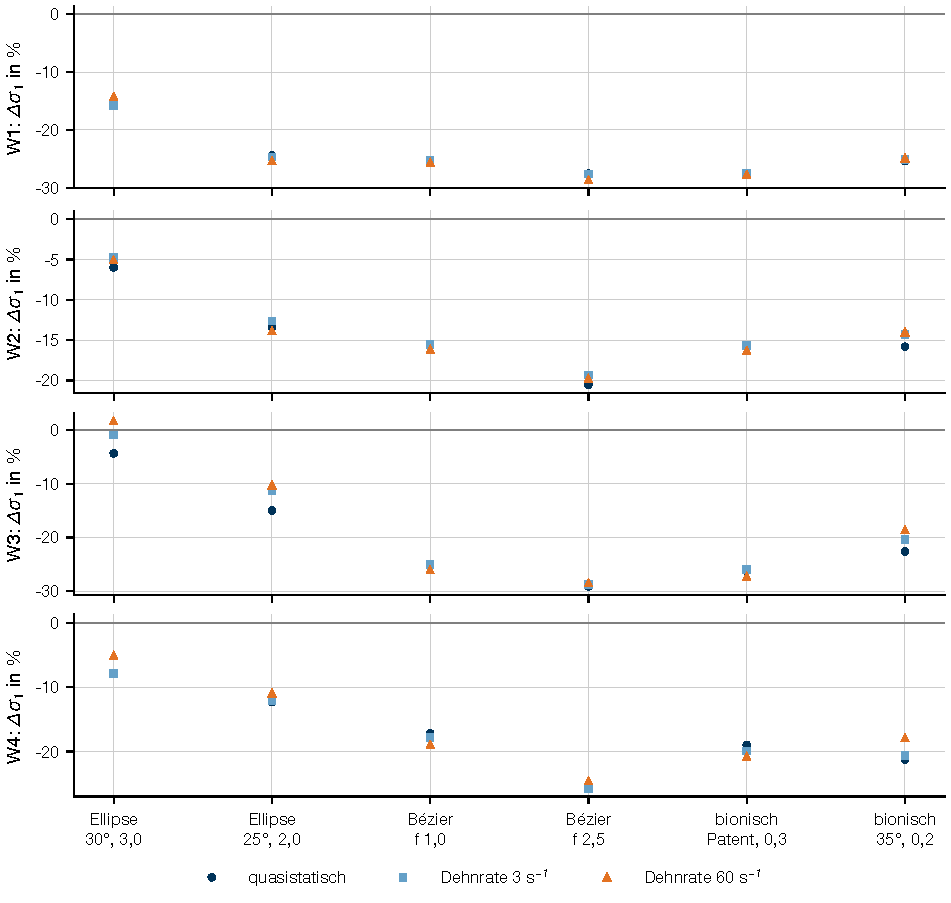
\includegraphics[width=0.95\textwidth]{kap5/fusseffekt_raten_16nm}
	\caption{Änderung der größten Zugspannung $\sigma_{\mathrm{1}}$ gegen die Trochoide am Normpunkt C je Variante, Werkstoffstufe (W1 bis W4 von oben nach unten) und Dehnratenkarte, Taschenkörper, $16$\,Nm. Marker ohne Linie.}
	\label{fig:fusseffekt_raten_16nm}
\end{figure}

Für den Nachweis nach Stommel et al. an der Fußrundung einer Variante ist die Lastgeschichte über alle Stellungen nötig. Die Grundserie des Taschenkörpers mit 99 Stellungen und W1 bis W4 bei quasistatischer Karte liegt vor und trägt den Nachweis in \secref{sec:stommel_ergebnis}. Die Vollserie des bionischen Optimums wurde zugunsten der Serien mit gemessener Geometrie zurückgestellt und bleibt Ausblick.

\subsection{Fertigungseinfluss der gemessenen Geometrie}
\label{sec:fussgeometrie_fertigung}

\begin{figure}[!htbp]
	\centering
	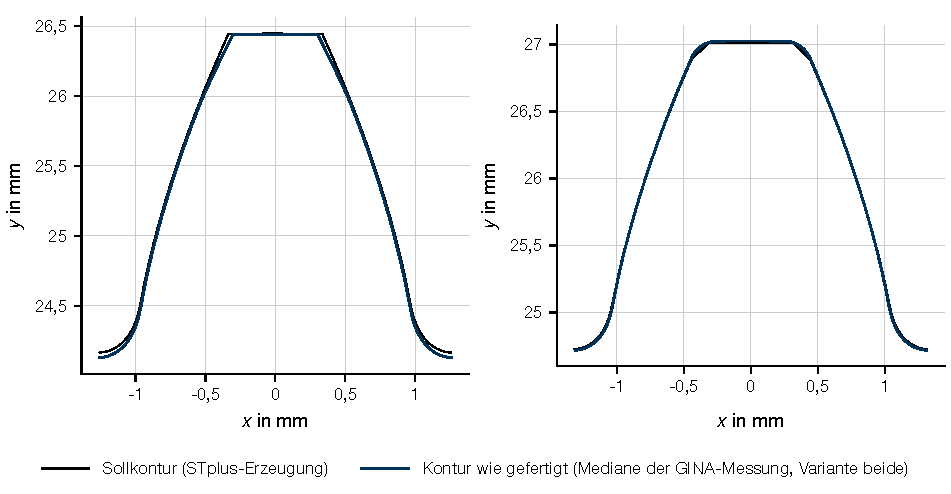
\includegraphics[width=0.95\textwidth]{kap5/kontur_zaehne_gemessen}
	\caption{Ritzel (links) und Rad (rechts) wie gefertigt gegen die STplus-Erzeugung, ganzer Zahn im Stirnschnitt in wahrem Maßstab. Mediane der GINA-Messung, Kopfrundung des Rades aus den Konturscans, Kopfrücknahme des Ritzels aus der GINA-Messung.}
	\label{fig:kontur_gemessen}
\end{figure}

Die Verzahnungsmessung in \secref{sec:pruefraeder_vorher} liefert die Abweichungen der gefertigten Teile von der Nenngeometrie, die Profil-Winkelabweichung, die Kopfrücknahme des Ritzels, die Kopfrundung des Rades von $0{,}21$\,mm und die Zahndicken. Daraus sind drei Rechenvarianten des Taschenkörpers aufgebaut: das Ritzel wie gemessen mit dem Rad der Nenngeometrie, das Rad wie gemessen mit dem Ritzel der Nenngeometrie und beide wie gemessen. Jede Variante trägt die Mediane der GINA-Messung über die Serie der Prüfstandsritzel und die Kernräder. Die Variante mit beiden Teilen wie gefertigt wurde als vollständige Serie über die 99 Stellungen mit W1 bis W4 und den drei Karten gerechnet. Das sind 1188 Rechnungen in $77{,}6$\,h mit drei Jobs zu je vier Kernen. Die beiden Einzelvarianten wurden an den Normpunkten A bis E gerechnet, je 60 Rechnungen in $3{,}7$ und $4{,}1$\,h. \figref{fig:kontur_gemessen} zeigt die gefertigten Zahnkonturen gegen die Erzeugung des STplus-Falls. Die Zahnweiten beider Teile treffen die STplus-Erzeugung der Nennserie, die das Zahndickenabmaß der Zeichnung schon trägt, am Ritzel auf $15$\,µm und am Rad auf $1$\,µm. Die Zahndicke ändert sich im Modell deshalb kaum. Am Ritzel liegt der Fußkreis $0{,}073$\,mm tiefer, und die lineare Kopfrücknahme nimmt ab dem Durchmesser $51{,}946$\,mm $23{,}6$\,µm zurück. Sie reicht auf der Eingriffslinie $1{,}15$\,mm vor E und erfasst damit den ganzen Doppeleingriff hinter D, wo sie noch $14$\,µm beträgt. Am Rad trägt die Profil-Winkelabweichung von $+10{,}25$\,µm Material zum Kopf hin auf, und der Bogen von $0{,}21$\,mm ersetzt die Fase der Erzeugung. Das Netz trägt drei Elementreihen auf dem Bogen und mit der Kopfkappe 87\,955 Knoten statt 83\,650. Die Normpunkte A bis E sind die der gefertigten Paarung mit der Profilüberdeckung $1{,}155$ gegen $1{,}154$ der Nenngeometrie.

\begin{figure}[!htbp]
	\centering
	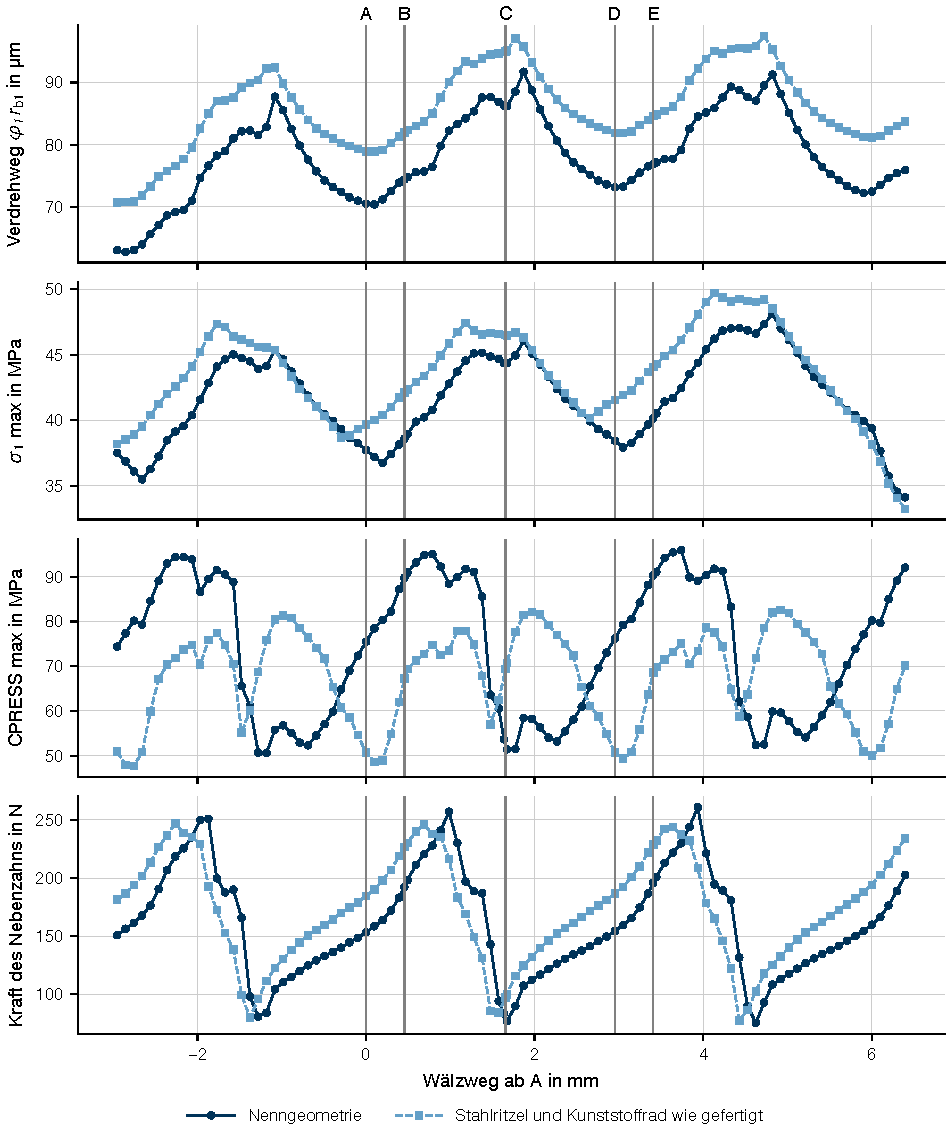
\includegraphics[width=0.95\textwidth]{kap5/vergleich_referenz_w2_12nm}
	\caption{Gefertigte Paarung gegen die Nenngeometrie über dem Wälzweg, W2, quasistatische Karte, $12$\,Nm, Größtwerte über die Zahnbreite: Verdrehwinkel, größte Zugspannung der Fußrundung, größter Kontaktdruck und die Kraft des Nebenzahns.}
	\label{fig:vergleich_referenz_w2_12nm}
\end{figure}

\begin{table}[!htbp]
	\caption{Gefertigte Paarung gegen die Nenngeometrie bei $12$\,Nm, quasistatische Karte, relative Änderung in \%: größte Zugspannung $\sigma_{\mathrm{1}}$ der Fußrundung im Maximum über dem Wälzweg und an B, C und E, größter Kontaktdruck $p_{\mathrm{max}}$ im Maximum und an C, Verdrehwinkel an C.}
	\label{tab:gemessen_vergleich}
	\centering
	\footnotesize
	\setlength{\tabcolsep}{4pt}
	\begin{tabular}{L{1.2cm}L{1.7cm}L{1.5cm}L{1.5cm}L{1.5cm}L{1.9cm}L{1.6cm}L{1.9cm}}
		Stufe & $\sigma_{\mathrm{1}}$ max & $\sigma_{\mathrm{1}}$ an B & $\sigma_{\mathrm{1}}$ an C & $\sigma_{\mathrm{1}}$ an E & $p_{\mathrm{max}}$ max & $p_{\mathrm{max}}$ an C & $\varphi_{\mathrm{1}}$ an C \\
		\hline
		\arrayrulecolor{black!30}
		W1    & $+7{,}3$            & $+22{,}6$            & $+6{,}9$             & $+20{,}5$            & $-31{,}2$        & $+24{,}5$         & $+8{,}7$              \\
		\hline
		W2    & $+3{,}3$            & $+9{,}2$             & $+4{,}8$             & $+9{,}8$             & $-14{,}0$        & $+29{,}3$         & $+10{,}0$             \\
		\hline
		W3    & $+9{,}5$            & $+19{,}6$            & $+7{,}5$             & $+20{,}7$            & $-31{,}0$        & $+25{,}1$         & $+8{,}7$              \\
		\hline
		W4    & $+6{,}2$            & $+11{,}5$            & $+2{,}2$             & $+10{,}7$            & $-20{,}9$        & $+15{,}4$         & $+9{,}6$              \\
		\hline
		\arrayrulecolor{black}
	\end{tabular}
\end{table}

\tabref{tab:gemessen_vergleich} stellt die Beanspruchung der gefertigten Paarung der Nenngeometrie bei $12$\,Nm gegenüber, \figref{fig:vergleich_referenz_w2_12nm} den Verlauf über dem Wälzweg für W2. Zwei Wirkungen überlagern sich. Die Kopfrücknahme des Ritzels mindert den Lastanteil des zweiten Zahnpaars an den Enden des Wälzwegs, die Kopfrundung des Rades in kleinerem Maß. Das Hauptpaar trägt an den Doppeleingriffspunkten einen größeren Teil der Last, und die Paarung wird nachgiebiger. Lastfrei wird das zweite Paar nicht, weil die Verformung der Paarung mit $90$ bis $150$\,µm über der Rücknahme liegt. Die Profilüberdeckung der unbelasteten Geometrie zeigt davon nichts, sie zählt die Evolventen bis zu den Kopfkreisen und steigt mit dem größeren Kopfkreis des Rades sogar leicht. Der Verdrehwinkel wächst im Maximum um $6$ bis $9$\,\% und an den Normpunkten A, B, D und E um $6$ bis $23$\,\%. Die größte Zugspannung der Fußrundung über dem Wälzweg steigt bei allen Stufen und Momenten um $3$ bis $10$\,\%. Die Kopfrücknahme des Ritzels nimmt dem Kantenkontakt am Eingriffsbeginn und am Eingriffsende die Schärfe, die Kopfrundung des Rades senkt den Druck an A und D um weitere $10$ bis $17$\,\%. Der Größtwert des Kontaktdrucks liegt bei der Nenngeometrie am Kantenkontakt der Ritzelkopfkante kurz hinter E, bei der gefertigten Paarung weiter außen im verlängerten Eingriff. Die beiden Größtwerte unterscheiden sich um $8$ bis $36$\,\%. An den festen Stellen B und E, wo die Nenngeometrie ihre höchsten Drücke hat, sinkt der Druck um $16$ bis $58$\,\%. Die Kraft des Nebenzahns im verlängerten Eingriff sinkt um $1$ bis $6$\,\%.

Am Wälzpunkt C liegt der Kontaktdruck bei $8$ und $12$\,Nm dagegen um $5$ bis $29$\,\% höher. Nach den Einzelvarianten stammt diese Erhöhung vom Ritzel, nicht von der Profil-Winkelabweichung des Rades. Die Kopfrücknahme nimmt dem Nebenzahn an C fast den ganzen Lastanteil, das Hauptpaar trägt $10$\,\% mehr, und der Verdrehwinkel wächst dort bei $12$\,Nm um $11$\,\%. Bei $16$\,Nm liegt der Kontaktdruck an C unter den plastischen Stufen um $7$ bis $16$\,\% niedriger. Die Zugspannung an C ändert sich um $-2$ bis $+8$\,\%, an B und E um $+5$ bis $+33$\,\%. Dort entlastet der weichere Kantenkontakt den Nebenzahn früher, und der Hauptzahn trägt mehr Last. Die Stufen unterscheiden sich in der Höhe, nicht im Vorzeichen. Die linearen Stufen W1 und W3 reagieren am stärksten, die plastischen Stufen W2 und W4 mindern den Zuwachs der Fußspannung um ein Sechstel bis zwei Drittel.

Nach den Einzelvarianten liegt die Änderung in der Mikrogeometrie des Ritzels. Das Ritzel allein erhöht bei $12$\,Nm die Zugspannung an C unter W1 um $7{,}6$\,\% und unter W2 um $4{,}7$\,\%. An B und E steigt sie um $7$ bis $18$\,\%, der größte Kontaktdruck sinkt um $21$ bis $32$\,\%. Das Rad allein ändert die Zugspannung an C um weniger als $1$\,\%, an B und E um $2$ bis $5$\,\% und den größten Kontaktdruck um $2$ bis $4$\,\%. Die Anteile überlagern sich an der Fußrundung bis auf einen Prozentpunkt additiv.

Der Nachweis nach Stommel et al. mit W2 auf der gefertigten Paarung findet seinen kritischen Knoten an derselben Stelle wie auf der Nenngeometrie. Er liegt in der Fußrundung zwischen T3 und T4 nahe der Stirnseite bei $z = -5{,}93$\,mm. Die zyklische Auslastung steigt von $1{,}30$, $1{,}64$ und $1{,}96$ auf $1{,}38$, $1{,}70$ und $2{,}00$. Die vorhergesagte Lastwechselzahl bis zum Anriss fällt bei $8$\,Nm von $1{,}7 \cdot 10^{5}$ auf $6{,}5 \cdot 10^{4}$ und bei $12$\,Nm von $4{,}3 \cdot 10^{3}$ auf $2{,}3 \cdot 10^{3}$, bei $16$\,Nm bleibt es beim sofortigen Versagen. Der statische Nachweis besteht weiterhin an allen Fußknoten. Mit der Karte DY2, die der Dehnrate des Prüfstands nach \secref{sec:stufen_raten_koerper} am nächsten liegt, sinkt die zyklische Auslastung auf $0{,}94$, $1{,}17$ und $1{,}33$. Bei $8$\,Nm besteht der Nachweis damit für $10^{7}$ Lastwechsel, und die vorhergesagte Lastwechselzahl bis zum Anriss von $3{,}5 \cdot 10^{7}$ liegt über der gemessenen Bruchlinie für $50$\,\% mit $2{,}7 \cdot 10^{7}$. Gegen die ersten sichtbaren Anrisse der beiden Räder dieser Stufe zwischen $3{,}2$ und $7{,}7 \cdot 10^{6}$ Lastwechseln (\secref{sec:versuchsprogramm}) liegt sie um den Faktor $5$ bis $11$ zu hoch. Bei $12$ und $16$\,Nm liegt sie mit $5{,}2 \cdot 10^{5}$ und $4{,}7 \cdot 10^{4}$ um die Faktoren $11$ und $29$ unter der Bruchlinie. Die Hill-Erweiterung verhält sich wie auf der Nenngeometrie. Unter W3 versagt der statische Nachweis an den Fußknoten jenseits der Isotherme. Unter W4 liegt der kritische Knoten in der Fußrundung zwischen T2 und T3 an derselben Stelle wie zuvor, mit einer zyklischen Auslastung von $2{,}57$ gegen $2{,}45$ bei $8$\,Nm.

% Herkunft:
% Absatz 1 und 2: 80_output/fe/kst_e/vergleich_fussrundung_AtoE/analyse.md Kopf und Abschnitt 1 (Konturen);
%   ADR-116 Punkt 52 und 53 (architecture_decisions.md); Tabelle 1: analyse.md Abschnitt 1 und
%   fussrundung_sweep/bericht.md (Spalte Δ der Literaturwerte und Optima).
% Tabelle 2 und Absatz "Reihenfolge": analyse.md Abschnitt 3.1 (Δσ1 an C, ΔDrehung an C) und 3.4 (eben gegen 3D).
% Absatz "Patentkonturen": analyse.md 3.1 (Spannen Δσ1 über A bis E, Δ|σ3|, ΔCPRESS) und Abschnitt 4 (16 Nm, Drehung und Kopfweg).
% Absatz "Ellipsen": analyse.md 3.1, 3.5 und 3.6 (Ort des Größtwerts r 24,48 bis 24,60 mm gegen 24,83 mm),
%   Abschnitt 4 (|σ3| W3_QS +46/+47 %, W3_DY1 +51 %); known_limits.md FE-25 (Netzgrenze).
% Absatz "Werkstoffstufen, Dehnraten und Last": analyse.md 3.1 (W2 gegen W1, W4 gegen W3), 3.2 (Raten), 3.3 (Lasten).
% Letzter Absatz: ADR-116 Punkt 53 (Kette: Grundserie und Vollserie des bionischen Optimums).
% Bildwunsch: Konturbild der sechs Fußrundungen gegen die Trochoide im Stirnschnitt (gearcore.fillet, noch zu zeichnen, T5).
% Nomenklatur: S_L (Lückenweite als Sehne am Übergangsdurchmesser, Patent DE 10 2008 045 318 B3) fehlt noch in nomenklatur.yaml.

\section{Vergleich der Berechnungsverfahren}
\label{sec:verfahrensvergleich}

\tabref{tab:verfahrensvergleich} stellt je Drehmomentstufe die Zahnfußspannung der Verfahren aus \secref{sec:analytik} und dem FE-Modell nebeneinander. Die Zahnfußspannung nach VDI 2736 Blatt 2 trägt die Faktoren $Y_{\mathrm{Fa}} = 2{,}211$ und $Y_{\mathrm{Sa}} = 1{,}904$ des STplus-Berichts für Kraftangriff am Kopf und $Y_{\varepsilon} = 0{,}900$. Daneben stehen die Werte von RIKOR und die größte Zugspannung $\sigma_{\mathrm{1}}$ des FE-Modells am Normpunkt C je Werkstoffstufe auf dem Taschenkörper aus \secref{sec:waelzweg}. Die letzten Spalten nennen die vorhergesagte Lastwechselzahl des Nachweises nach Stommel et al. mit W2 aus \secref{sec:stommel_ergebnis} und die gemessene Bruchlinie aus \secref{sec:woehlerlinien}.

\begin{table}[htbp]
	\caption{Zahnfußspannung je Drehmomentstufe nach Verfahren in MPa und Lastwechselzahlen: Zahnfußspannung nach VDI 2736 Blatt 2, RIKOR N 3.0 linear elastisch mit $E = 2282$\,MPa wie W1, FE-Modell am Normpunkt C je Werkstoffstufe (Taschenkörper, quasistatisch), vorhergesagte Lastwechselzahl nach Stommel et al. mit W2 und gemessene Lastwechselzahl für $50$\,\% Ausfallwahrscheinlichkeit.}
	\label{tab:verfahrensvergleich}
	\centering
	\footnotesize
	\setlength{\tabcolsep}{4pt}
	\begin{tabular}{L{1.0cm}L{1.6cm}L{1.2cm}L{1.0cm}L{1.0cm}L{1.0cm}L{1.0cm}L{1.7cm}L{1.7cm}}
		$T_{2}$ in Nm & $\sigma_{\mathrm{F}}$ nach VDI 2736 & RIKOR    & FE W1    & FE W2    & FE W3    & FE W4    & $N_{\mathrm{pred}}$ W2 & $N_{\mathrm{L},50\%}$ \\
		\hline
		\arrayrulecolor{black!30}
		$8$           & $77{,}7$                            & $56{,}6$ & $59{,}4$ & $38{,}8$ & $57{,}6$ & $44{,}3$ & $1{,}7 \cdot 10^{5}$   & $2{,}67 \cdot 10^{7}$ \\
		\hline
		$12$          & $116{,}6$                           & $73{,}3$ & $72{,}7$ & $44{,}4$ & $71{,}0$ & $52{,}0$ & $4{,}3 \cdot 10^{3}$   & $5{,}96 \cdot 10^{6}$ \\
		\hline
		$16$          & $155{,}4$                           & $91{,}3$ & $86{,}2$ & $50{,}0$ & $84{,}6$ & $59{,}8$ & sofort                 & $1{,}36 \cdot 10^{6}$ \\
		\hline
		\arrayrulecolor{black}
	\end{tabular}
\end{table}

Die FE-Spannung am Normpunkt C wächst mit dem Moment unterproportional. Von $8$ auf $16$\,Nm verdoppelt sich die Umfangskraft, die Zugspannung steigt bei W1 um den Faktor $1{,}45$, bei W2 um $1{,}29$, bei W3 um $1{,}47$ und bei W4 um $1{,}35$. Der Grund liegt in der Lastaufteilung des verformten Zahns, bei den plastischen Stufen zusätzlich im Fließen. Die Zahnfußspannung nach VDI 2736 Blatt 2 wächst dagegen proportional zur Umfangskraft, weil ihre Faktoren nur von der Geometrie abhängen. Sie liegt über jeder FE-Stufe, bei $8$\,Nm um den Faktor $1{,}3$ gegen W1 und $2{,}0$ gegen W2, bei $16$\,Nm um $1{,}8$ und $3{,}1$. RIKOR rechnet mit demselben Modul von $2282$\,MPa wie die Stufe W1 und trifft deren Zugspannung an C innerhalb von $-5$ bis $+6$\,\%, bei $8$\,Nm darunter, bei $16$\,Nm darüber. Trägt man die gemessenen Lastwechselzahlen der $50$\,\%-Linie über der Spannung jedes Verfahrens auf, folgt aus den Werten der Tabelle die Neigung $k$ einer lokalen Wöhlerlinie je Verfahren (\tabref{tab:neigung_verfahren}). Die Zahnfußspannung nach der Richtlinie gibt mit $4{,}3$ fast die Neigung $4{,}40$ der Momentlinie wieder, RIKOR $6{,}2$, die elastischen FE-Stufen $7{,}7$ bis $8{,}0$ und die plastischen Stufen $10$ bis $13$. Die Dehnratenkarten ändern die Neigung über $8$ bis $16$\,Nm um höchstens zwei Einheiten, krümmen die Linie aber, weil die Spannung bei DY2 von $8$ auf $12$\,Nm stärker wächst als von $12$ auf $16$\,Nm. Diese Linien sind keine Werkstoffkennlinien, sondern die gemessene Bruchlinie, über die Spannung des jeweiligen Verfahrens aufgetragen. Mit ihnen wird in \secref{sec:genauigkeit} die synthetische Wöhlerlinie des Nachweises eingeordnet.

\begin{table}[htbp]
	\caption{Neigung $k$ der gemessenen Bruchlinie für $50$\,\% über der Zahnfußspannung des jeweiligen Verfahrens, aus den Spannungen bei $8$ und $16$\,Nm. FE am Normpunkt C des Taschenkörpers je Werkstoffstufe und Dehnratenkarte.}
	\label{tab:neigung_verfahren}
	\centering
	\footnotesize
	\begin{tabular}{L{3.2cm}L{1.2cm}L{1.2cm}L{1.2cm}L{1.2cm}}
		Verfahren                                  & W1                                & W2       & W3      & W4       \\
		\hline
		\arrayrulecolor{black!30}
		FE, Karte QS                               & $8{,}0$                           & $11{,}8$ & $7{,}7$ & $10{,}0$ \\
		\hline
		FE, Karte DY1                              & $8{,}0$                           & $13{,}2$ & $8{,}0$ & $10{,}4$ \\
		\hline
		FE, Karte DY2                              & $6{,}4$                           & $12{,}0$ & $6{,}6$ & $10{,}6$ \\
		\hline
		VDI 2736 Blatt 2                           & \multicolumn{4}{l}{$4{,}3$}                                       \\
		\hline
		RIKOR                                      & \multicolumn{4}{l}{$6{,}2$}                                 \\
		\hline
		Raddrehmoment (\secref{sec:woehlerlinien}) & \multicolumn{4}{l}{$4{,}40$}                                      \\
		\arrayrulecolor{black}
		\hline
	\end{tabular}
\end{table}

% TK erledigt (2026-10-25: RIKOR N 3.0 von der Betreuerin mit E 2282 MPa der QS-Karte neu gerechnet, Werte 56,6/73,3/91,3 MPa vom Nutzer eingetragen; Text, Unterschrift, Neigung 6,2 und Kapitel 7 nachgezogen): Workbench Vergelich habe ich rausgenommen, da da kein wesentlicher Unterschied noch nennenswert ist. Entsrpechend noch die VDI Kette und Rikor wurde mit 3900 MPa linear elastisch gerechnet. Was hatte unsere W1 zugrundegelegt? Wäre da das gleiche E-Modul und gleiche Qerkontraktion nochmal sinnvoll? 

% Herkunft:
% FE-Werte an C: series analyse.md Abschnitt 2 (σ1 C: W1 56,09/70,43/82,87, W2 38,27/43,74/48,90, W3 65,07/81,87/
%   97,35, W4 48,58/56,92/65,23); Faktoren 16 gegen 8 Nm: 82,87/56,09 = 1,48, 48,90/38,27 = 1,28, 97,35/65,07 =
%   1,50, 65,23/48,58 = 1,34; N_pred: analyse.md Abschnitt 7 (W2 3,54e5/2,24e4/1,65e3); N_L,50 %: woehler.md.
%   RIKOR gegen W1: 56,6/59,4 = 0,953, 73,3/72,7 = 1,008, 91,3/86,2 = 1,059; VDI gegen RIKOR 1,37/1,59/1,70;
%   Neigung RIKOR lg(2,67e7/1,36e6)/lg(91,3/56,6) = 1,293/0,208 = 6,2 (2026-10-25).
%   VDI 2736: Y_Fa/Y_Sa offen (L6b, kap3_4); RIKOR/Workbench: Nutzer liefert 2026-10-19 (L6a); Bild L8 und Skript
%   root_stress_comparison.py (C7) folgen.
% Bildwunsch: L8-Bild nach C7.
% Bibwunsch: keiner.
% Nomenklatur: sigma_F, N_pred, N_L.
% Offen: alle Platzhalter dieses Abschnitts.
